\chapter{Thực nghiệm và đánh giá}\label{chap:eval}

Chương này trả lời câu hỏi: gia sư CAVAT hiện thực được những thiết kế nào và mạnh hơn, hoặc không mạnh hơn, chatbot thông thường ở điểm nào. Chương dùng hai loại bằng chứng, nhật ký các buổi học thử nghiệm trên hệ thống và các bộ câu hỏi, tình huống soạn sẵn để so sánh có kiểm soát, và trả lời năm câu hỏi nghiên cứu ở Bảng~\ref{tab:rq}: phương pháp đánh giá (mục~\ref{sec:eval-method}), truy xuất (mục~\ref{sec:eval-rag}), hành vi so với chatbot và việc chấm (mục~\ref{sec:eval-socratic} và \ref{sec:eval-grading}), mức hiểu (mục~\ref{sec:eval-learner}) và bộ chọn nước đi (mục~\ref{sec:eval-bandit}). Mọi con số được báo như đã đo, kể cả khi hệ thống không hơn đối chứng.

\section{Phương pháp đánh giá}\label{sec:eval-method}

\subsection{Hai nguồn dữ liệu}
Nguồn thứ nhất là nhật ký các buổi học thử nghiệm thật, đọc từ bản sao lưu cơ sở dữ liệu ngày 16/11/2026 bằng một lệnh chỉ đọc. Bản sao gồm $43$ buổi của năm tài khoản học sinh thử nghiệm với $14\,078$ sự kiện; mỗi sự kiện ghi một việc đã xảy ra (học sinh nhập phản hồi, gia sư đưa gợi ý, bộ chấm trả kết quả) và chỉ được bổ sung, không bị sửa. Tài khoản Vuong chiếm $79{,}7\%$ số sự kiện và $92{,}7\%$ số câu hỏi đã hiển thị ($523$ trên $564$ câu) vì học nhiều nhất, nên các mục kết quả lấy tài khoản này làm nguồn chính: $12$ buổi có ít nhất một câu được giải quyết, gồm sáu buổi Toán chương Số thập phân, bốn buổi Toán chương Diện tích và hai buổi Tiếng Anh Unit~11. Bốn tài khoản còn lại chỉ góp vào các phép đếm về mô hình ngôn ngữ và bộ kiểm chứng ở mục~\ref{sec:eval-model}, nơi kết quả không phụ thuộc vào việc ai học. Các số liệu được tính lại bằng chương trình đọc nhật ký và chỉ xuất số liệu tổng hợp, không xuất phản hồi học sinh hay tên tài khoản.

Nguồn thứ hai là các bộ câu hỏi và tình huống soạn sẵn, được lưu lại bằng thẻ git trước khi sửa phần hệ thống mà chúng đo, gọi là \emph{đóng băng}. Bộ đóng băng cho phép so sánh công bằng giữa các cách làm. Bảng~\ref{tab:eval-sets} liệt kê các bộ, do ai viết, dùng để làm gì và có độc lập với thiết kế không; điều này quyết định bộ nào được dùng làm bằng chứng kết luận.

\begin{table}[H]
\centering
\caption{Các bộ dữ liệu đánh giá. Bộ độc lập là bộ chưa từng được xem để sửa thiết kế. Nhãn truy xuất là mọi đoạn của bài trả lời câu hỏi, do người phát triển và một trợ lý AI soạn, chưa có chuyên gia thẩm định.}\label{tab:eval-sets}
\small
\begin{tabular}{>{\raggedright\arraybackslash}p{2.7cm}r>{\raggedright\arraybackslash}p{5.2cm}>{\raggedright\arraybackslash}p{4.3cm}}
\toprule
Bộ & Cỡ mẫu & Nội dung và cách dựng & Độc lập với thiết kế? \\
\midrule
Bộ chỉnh & $30$ (trong bài $18$) & Câu hỏi truy xuất dùng để chỉnh ngưỡng định tuyến & Không \\
Bộ 1 & $23$ ($14$) & Viết sau bộ chỉnh; các câu trượt đã được đọc khi thiết kế định tuyến & Không \\
Bộ 2 & $30$ ($20$) & Viết sau khi thiết kế xong, nhiều câu hỏi bài trước hơn ($12$ so với $7$) vì định tuyến nhắm vào loại câu này; đóng băng trước khi sửa mã & Có \\
Bộ 3 & $43$ ($30$) & Câu viết như trẻ gõ không dấu, viết tắt; dùng để sửa ở lần cải tiến cuối & Không \\
Bộ 4 & $37$ ($22$) & Câu viết như trẻ gõ; đóng băng trước lần cải tiến cuối & Có \\
$13$ vai học sinh khó & $31$ lượt & Kịch bản hội thoại nhóm soạn, một bài tập & Có \\
Bộ chấm 1 và 2 & $36$ và $35$ câu & Câu trả lời điển hình của trẻ, gán nhãn đúng sai bằng tay & Bộ 2 độc lập; Bộ 1 đã xem khi sửa \\
Chuỗi sự kiện & $2\times500$ & Chuỗi ngẫu nhiên kiểm công thức mức hiểu & Có \\
\bottomrule
\end{tabular}
\end{table}

Vì Bộ chỉnh, Bộ 1 và Bộ 3 không độc lập, kết luận về truy xuất dựa chủ yếu vào Bộ 2 và Bộ 4; các bộ kia chỉ cho thấy chiều của tác dụng. Mô hình nhúng \texttt{gemini-embedding-001} đo độ gần về nghĩa, khoảng tin cậy tính bằng lấy mẫu lại $10\,000$ lần, kiểm định McNemar so hai cách chạy trên cùng một bộ câu, và khoảng Wilson $95\%$ cho các tỉ lệ nhỏ.

\subsection{Các chỉ số dùng trong chương}
Hit@3 là tỉ lệ câu hỏi mà đoạn đúng nằm trong ba kết quả đầu; MRR là trung bình của $1/\text{thứ hạng}$ của đoạn đúng đầu tiên (luôn đứng đầu thì bằng $1$, không có thì bằng $0$). Hit@3 và MRR chỉ tính trên các câu có đoạn đúng trong kho, tức câu về bài đang học và bài trước. Độ gần cosine đo hai đoạn văn giống nhau về nghĩa trong khoảng từ $0$ đến $1$. Khoảng tin cậy $95\%$ là khoảng mà giá trị thật nhiều khả năng nằm trong. $p$ của kiểm định McNemar cho biết chênh lệch giữa hai cách chạy có thể chỉ do ngẫu nhiên hay không; $p<0{,}05$ nghĩa là chênh lệch khó là ngẫu nhiên. Điểm hiểu bài $M$ từ $0$ đến $100$ ước lượng học sinh hiểu một bài đến đâu, kèm mức hiểu từ $0$ đến $5$. Hối tiếc tích lũy của bộ chọn nước đi là tổng phần thưởng bị mất so với luôn chọn nước tốt nhất. Một câu có bốn cách kết thúc: \emph{tự làm} (đúng không cần gợi ý), \emph{có gợi ý} (đúng sau một đến năm bậc), \emph{làm mẫu} (phải đến bậc sáu hoặc bảy) và \emph{chưa giải quyết}.

\subsection{Phạm vi của các kết luận}
Các số trong chương đo cách hệ thống hoạt động, không đo hiệu quả học tập của trẻ em. Các buổi do nhóm phát triển thực hiện bằng tài khoản học sinh thử nghiệm Vuong, chưa có trẻ em tham gia, và các buổi Toán tháng 10 chạy trên những bản gia sư cũ hơn bản đang triển khai. Chương vì thế chỉ kết luận về hai điều: hệ thống có giữ các quy tắc đã đặt không, và nó khác chatbot thông thường ra sao trong cùng tình huống.

\section{Kết quả thử nghiệm thực tế trên tài khoản học sinh Vuong}\label{sec:eval-trial}

Mục này đọc nhật ký tài khoản Vuong để trả lời: học sinh đã làm bao nhiêu câu, các câu kết thúc ra sao, gia sư đã giúp bao nhiêu và vòng dạy có chạy đủ các bước không. Bảng~\ref{tab:db-overview} cho quy mô trên các buổi có ít nhất một câu được hiển thị: tài khoản học $523$ câu và gửi $726$ câu trả lời đã chấm, trong đó Toán chiếm $89{,}9\%$ số câu. Chín trong mười buổi Toán diễn ra trong hai ngày 12 và 13/10, khi chủ dự án cho tài khoản học hết các tình huống của hai chương; hai buổi Tiếng Anh cách đó một tháng, sau khi môn thứ ba được thêm vào hệ thống.

% Sinh bởi tools/db_tex.py từ bản sao lưu database; không sửa tay.
\begin{table}[H]
\centering
\caption{Quy mô dữ liệu thử nghiệm đọc từ database}\label{tab:db-overview}
\begin{tabular}{lrrr}
\toprule
Chỉ số & Số thập phân & Diện tích & Tiếng Anh \\
\midrule
Số buổi học đã ghi & $10$ & $6$ & $5$ \\
Số buổi có nội dung & $6$ & $4$ & $3$ \\
Số buổi đã hoàn thành & $5$ & $3$ & $2$ \\
Số tài khoản thử nghiệm & $1$ & $1$ & $1$ \\
Số sự kiện & $5\,791$ & $3\,528$ & $1\,906$ \\
Số câu hỏi đã hiển thị & $287$ & $183$ & $53$ \\
Số lượt trả lời đã chấm & $401$ & $251$ & $74$ \\
Số câu đã giải quyết & $286$ & $182$ & $52$ \\
\bottomrule
\end{tabular}
\end{table}


\subsection{Các câu kết thúc ra sao}
Bảng~\ref{tab:db-results} và Hình~\ref{fig:db-resolution} cho cách các câu kết thúc. Học sinh tự làm được $58{,}4\%$ số câu ở chương Số thập phân, $64{,}3\%$ ở chương Diện tích và $76{,}9\%$ ở Unit~11. Phần còn lại chủ yếu được giải quyết sau gợi ý ($32{,}9\%$, $30{,}2\%$ và $19{,}2\%$) và chỉ một phần nhỏ phải làm mẫu ($5{,}6\%$, $3{,}8\%$ và $1{,}9\%$). Câu chưa giải quyết chỉ chiếm $3{,}1\%$, $1{,}6\%$ và $1{,}9\%$, nên gia sư đưa gần mọi câu đến đáp án đúng, có hoặc không có giúp đỡ. Số gợi ý trung bình cho mỗi câu giảm từ $0{,}71$ ở Số thập phân xuống $0{,}54$ ở Diện tích và $0{,}52$ ở Unit~11.

% Sinh bởi tools/db_tex.py từ bản sao lưu database; không sửa tay.
\begin{table}[H]
\centering
\caption{Cách giải quyết câu và kết quả chấm từng lượt trả lời}\label{tab:db-results}
\begin{tabular}{lrrr}
\toprule
Chỉ số & Số thập phân & Diện tích & Tiếng Anh \\
\midrule
Tự làm & $167$ ($58{,}4$\%) & $117$ ($64{,}3$\%) & $40$ ($76{,}9$\%) \\
Có gợi ý & $94$ ($32{,}9$\%) & $55$ ($30{,}2$\%) & $10$ ($19{,}2$\%) \\
Làm mẫu & $16$ ($5{,}6$\%) & $7$ ($3{,}8$\%) & $1$ ($1{,}9$\%) \\
Chưa giải quyết & $9$ ($3{,}1$\%) & $3$ ($1{,}6$\%) & $1$ ($1{,}9$\%) \\
\midrule
Đúng & $273$ ($68{,}1$\%) & $179$ ($71{,}3$\%) & $50$ ($67{,}6$\%) \\
Đúng một phần & $0$ ($0{,}0$\%) & $0$ ($0{,}0$\%) & $3$ ($4{,}1$\%) \\
Sai & $128$ ($31{,}9$\%) & $72$ ($28{,}7$\%) & $21$ ($28{,}4$\%) \\
\midrule
Số lần thử trung bình mỗi câu & $1{,}40$ & $1{,}37$ & $1{,}42$ \\
Số gợi ý trung bình mỗi câu & $0{,}71$ & $0{,}54$ & $0{,}52$ \\
\bottomrule
\end{tabular}
\end{table}


\begin{figure}[H]
\centering
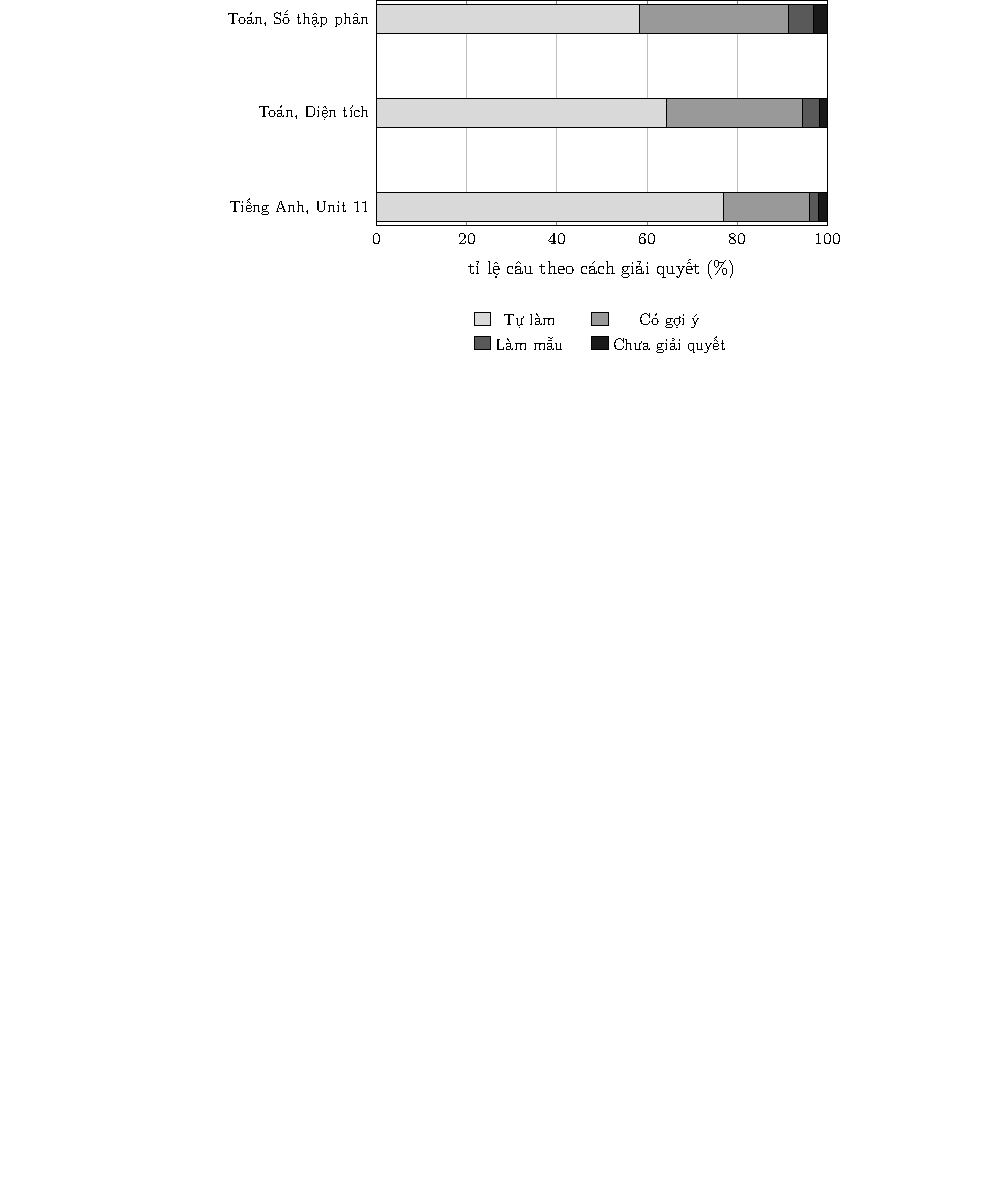
\includegraphics{figures/pdf/fig-db-resolution.pdf}
\caption{Tỉ lệ câu theo cách kết thúc của tài khoản Vuong ở ba nội dung. Mỗi thanh cộng lại bằng $100\%$.}
\label{fig:db-resolution}
\end{figure}

Hình~\ref{fig:db-curve} vẽ tỉ lệ câu tự làm của từng buổi từ tám câu trở lên theo thứ tự thời gian. Chương Diện tích tăng đều từ $41{,}7\%$ ở buổi đầu lên $53{,}7\%$, $70{,}7\%$ và $72{,}4\%$ ở ba buổi sau. Chương Số thập phân đi từ $52{,}4\%$ ở buổi hoàn chỉnh đầu tiên lên $66{,}7\%$ ở buổi thứ năm rồi giảm xuống $51{,}5\%$ ở buổi cuối; buổi cuối chỉ có $33$ câu nên dao động lớn và số liệu không đủ để nói nguyên nhân. Hai buổi Tiếng Anh có mức tự làm cao ngay từ đầu ($78{,}0\%$ và $72{,}7\%$) nhưng chỉ có $41$ và $11$ câu nên chưa so được với Toán.

\begin{figure}[H]
\centering
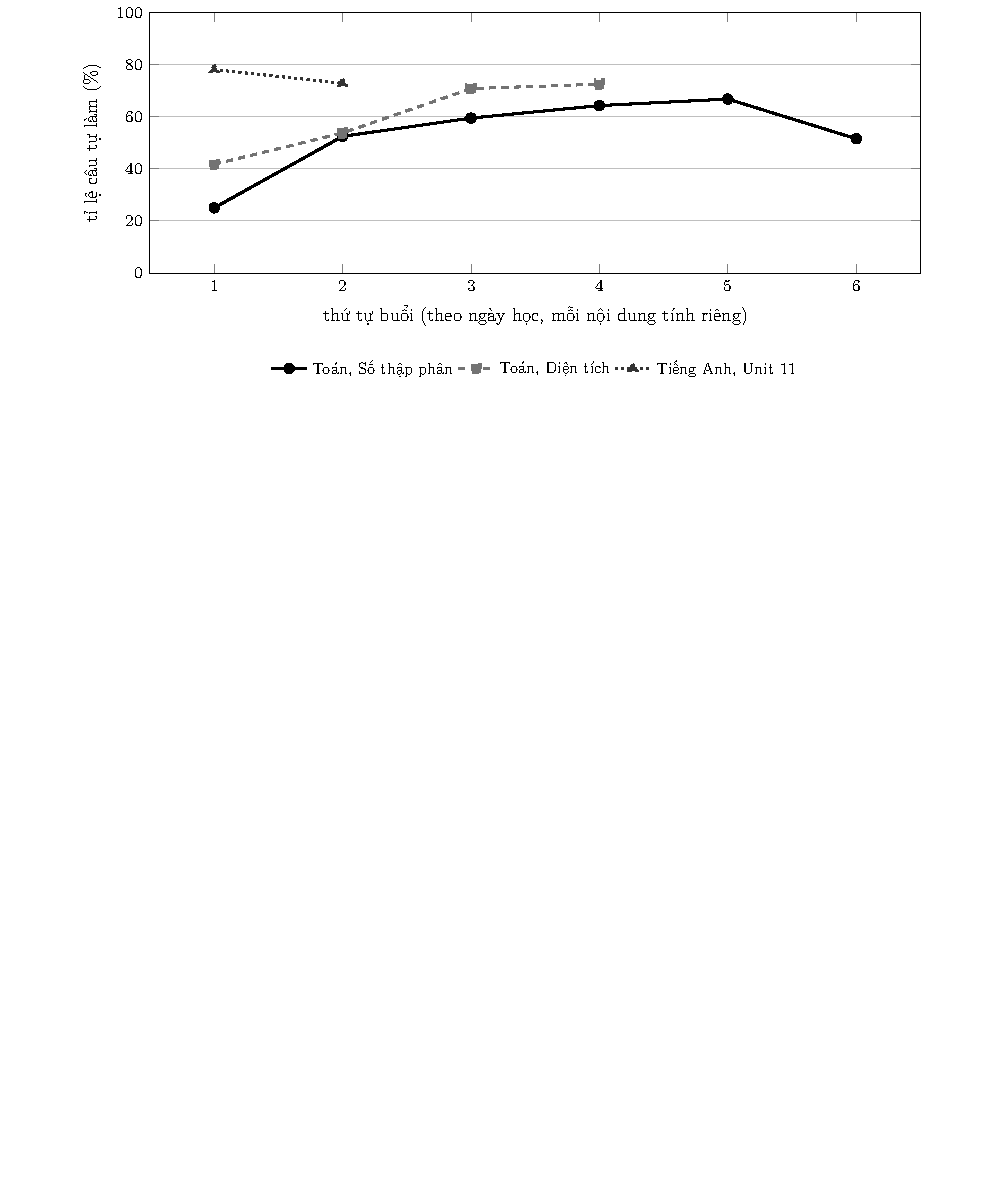
\includegraphics{figures/pdf/fig-db-curve.pdf}
\caption{Tỉ lệ câu tự làm của tài khoản Vuong theo thứ tự buổi, mỗi nội dung một đường; chỉ tính các buổi từ tám câu trở lên.}
\label{fig:db-curve}
\end{figure}

\subsection{Gợi ý theo bậc và vòng dạy}
Gợi ý tập trung ở bậc thấp, đúng nguyên tắc Socratic. Môn Toán có $295$ gợi ý: $62{,}7\%$ ở bậc một, $19{,}7\%$ ở bậc hai, $4{,}4\%$ ở bậc ba và $13{,}2\%$ là làm mẫu (bậc sáu và bảy); chỉ khoảng một trong tám gợi ý đi đến làm mẫu. Môn Tiếng Anh có $28$ gợi ý trải đều hơn trên các bậc một đến ba. Học sinh chủ động xin gợi ý $37$ lần ở Số thập phân, $16$ lần ở Diện tích và $10$ lần ở Unit~11, ít hơn tổng gợi ý đã đưa, nên phần lớn gợi ý do chính sách quyết định chứ không do học sinh đòi. Về vòng dạy, học sinh vào bài $47$ lần và qua bài $44$ lần ($93{,}6\%$) ở Số thập phân, vào $27$ lần và qua $26$ lần ($96{,}3\%$) ở Diện tích; Tiếng Anh qua $6$ trên $9$ lần vào bài, mẫu quá nhỏ và là buổi đầu của một môn mới đang sửa lỗi. Các quyết định dạy lý thuyết, hỏi kể lại, làm mẫu và đưa câu luyện tập xuất hiện đủ trong nhật ký cả hai môn, nên vòng sáu bước chạy trọn vẹn thay vì rút gọn thành một chuỗi câu hỏi.

\section{Mô hình ngôn ngữ và bộ kiểm chứng trong thực tế}\label{sec:eval-model}
Mục này đếm hoạt động của mô hình ngôn ngữ và bộ kiểm chứng trên cả năm tài khoản. Nó cũng trả lời một câu hỏi của việc đánh giá: mô hình ngôn ngữ thực sự viết bao nhiêu phần phản hồi, khi mỗi nước đi còn có câu mẫu của giáo viên làm dự phòng.

Hình~\ref{fig:db-source} cho biết mỗi phản hồi của gia sư do ai viết: mô hình, câu mẫu của giáo viên hay câu dự phòng khi không có gợi ý hợp lệ. Ở các buổi Toán đầu tháng 10 của Vuong, mô hình chỉ viết $2{,}1\%$ số phản hồi, còn $85{,}6\%$ là câu mẫu và $12{,}3\%$ là câu dự phòng, vì khi đó bộ diễn đạt còn là phiên bản cũ. Tỉ lệ này lên $40{,}9\%$ ở các buổi Toán cuối tháng 10 của những tài khoản khác, sau các đợt cải tiến lời dạy. Ở Tiếng Anh, mô hình viết $34{,}8\%$ phản hồi lần học đầu ngày 15/11 và $68{,}2\%$ lần sau khi sửa chuỗi mô hình và hạn mức gọi. Đây là câu trả lời cho thắc mắc rằng phần lớn lượt dùng câu mẫu chuẩn của giáo viên: điều đó đúng ở bản diễn đạt cũ, và phần của mô hình đã tăng ở các bản sau; câu mẫu vẫn là tuyến dự phòng cuối nên tỉ lệ do mô hình viết không bao giờ đến $100\%$, và đó là chủ ý thiết kế. Trong $13$ kịch bản có kiểm soát ở mục~\ref{sec:eval-socratic}, mô hình viết $26$ trong $31$ lượt ($84\%$) của CAVAT, còn $5$ lượt (nêu đề và đóng câu hỏi) luôn dùng câu mẫu theo thiết kế.

\begin{figure}[H]
\centering
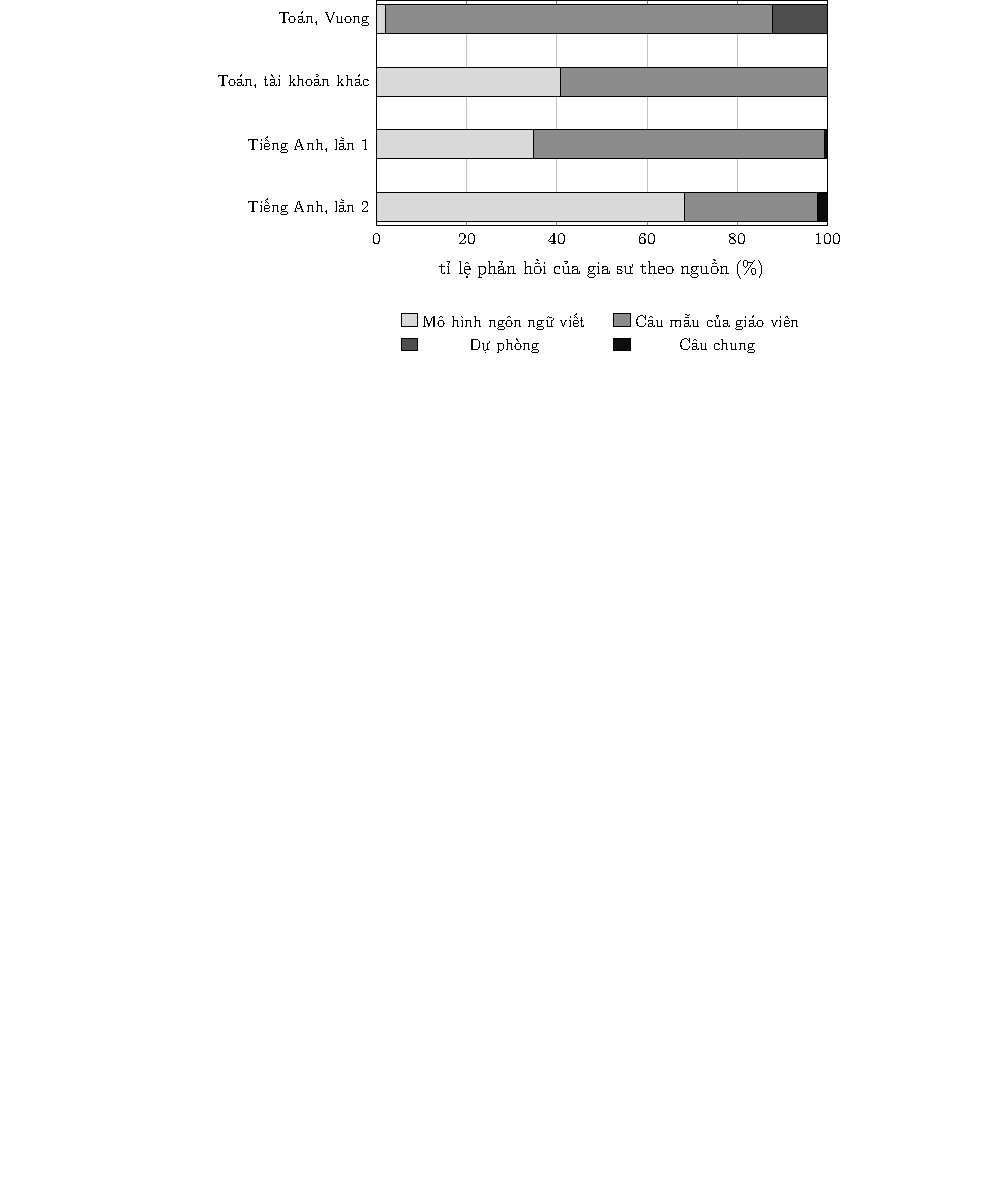
\includegraphics{figures/pdf/fig-db-source.pdf}
\caption{Tỉ lệ phản hồi của gia sư theo nguồn ở bốn nhóm buổi: Toán của Vuong (đầu tháng 10), Toán của bốn tài khoản khác (cuối tháng 10) và hai lần học Tiếng Anh của Vuong ngày 15/11.}
\label{fig:db-source}
\end{figure}

Bốn mô hình nhận $735$ lần gọi: gpt-oss-120b nhiều nhất ($337$ lần), tiếp đến Qwen ($219$), gpt-oss-20b ($155$) và Gemini ($24$); số token vào trung bình mỗi lần gọi từ $1\,321$ đến $1\,753$, thấp hơn nhiều giới hạn $3\,000$. Trong $1\,604$ lần chuyển sang mô hình kế tiếp, nguyên nhân là hết hạn mức ($71{,}1\%$), mô hình không phản hồi ($27{,}9\%$) và chỉ $1{,}0\%$ do kết quả không hợp lệ. Vấn đề chính của chuỗi mô hình vì vậy là hạn mức miễn phí chứ không phải chất lượng đầu ra, và điều đó biện minh cho chuỗi có dự phòng. Về bộ kiểm chứng, Bảng~\ref{tab:db-rejected} đếm lý do từ chối: ở Toán là phản hồi quá dài ($30$ lần), thiếu câu hỏi ($10$) và xưng hô sai ($10$); ở Tiếng Anh là từ tiếng Anh ngoài tư liệu ($20$), lộ đáp án ($8$), nhiều hơn một câu hỏi ($6$) và thiếu câu hỏi ($6$). Tám lần lộ đáp án bị chặn và không lần nào đến học sinh. Hai dòng đầu của bảng ($24$ lần hết số lần gọi và $22$ lần mô hình vẫn không qua kiểm chứng) là các lần hệ thống bỏ lời của mô hình để dùng câu mẫu, nên đo mức rơi về tuyến dự phòng chứ không đo lỗi của gia sư.

% Sinh bởi tools/db_tex.py từ bản sao lưu database; không sửa tay.
\begin{table}[H]
\centering
\caption{Lý do bộ kiểm chứng từ chối phản hồi của gia sư}\label{tab:db-rejected}
\begin{tabular}{lrr}
\toprule
Lý do từ chối & Toán & Tiếng Anh \\
\midrule
quá dài & $30$ & $0$ \\
hết số lệnh gọi của buổi & $0$ & $24$ \\
mô hình vẫn không qua kiểm chứng & $0$ & $22$ \\
từ tiếng Anh ngoài tư liệu của bài & $0$ & $20$ \\
thiếu câu hỏi & $10$ & $6$ \\
xưng hô sai & $10$ & $0$ \\
lộ đáp án & $0$ & $8$ \\
nhiều hơn một câu hỏi & $0$ & $6$ \\
từ ngoài tư liệu của câu & $0$ & $1$ \\
khen trí thông minh & $0$ & $1$ \\
\bottomrule
\end{tabular}
\end{table}


\section{Kết quả truy xuất tài liệu}\label{sec:eval-rag}

Gia sư tìm trong kho tài liệu của giáo viên những đoạn để dựa vào khi học sinh hỏi. Mục này đo ba điều: hệ thống có tìm đúng đoạn không, thành phần nào đóng góp nhiều nhất, và cách tìm có ràng buộc theo thứ tự bài học có tránh được việc dạy trước nội dung chưa học không. Kho gồm $221$ đoạn của hai chương Toán, mỗi đoạn gắn với bài của nó. Năm bộ câu hỏi ở Bảng~\ref{tab:eval-sets} có bốn loại câu: về bài đang học, về bài trước, về bài sau mà học sinh chưa học, và Toán ngoài chương hoặc lạc đề. Phép đo dừng ở chỗ đoạn nào được tìm ra, chưa đo chất lượng câu trả lời cuối cùng mà học sinh đọc.

\subsection{Mỗi thành phần đóng góp bao nhiêu}
Hình~\ref{fig:rag-hit3} so sáu cách tìm. Ba cách đầu, gồm tìm theo từ khóa, theo vector và tìm lai, gần như giống nhau: ở Bộ 2 cả ba cho Hit@3 bằng $0{,}40$ và MRR từ $0{,}449$ đến $0{,}460$. Nguyên nhân nằm ở dữ liệu: văn bản của giáo viên ngắn và dùng chung nhiều thuật ngữ giữa các bài (``phần nguyên'', ``hàng'', ``dấu phẩy''), nên đoạn của bài đang học và của bài khác khớp từ khóa và nghĩa gần như nhau. Điều phân biệt hai loại đoạn là cấu trúc, tức học sinh đang ở bài nào. Cấu hình của đồ án, tức tìm lai kèm các bước dựa vào thứ tự bài học, đạt MRR $0{,}954$ ở Bộ 2 và $0{,}935$ ở Bộ 4, so với $0{,}460$ và $0{,}343$ của tìm lai thuần; ở Bộ 2 mức tăng là $0{,}494$ (khoảng tin cậy từ $0{,}306$ đến $0{,}678$), với mười một câu chuyển từ sai sang đúng và không câu nào ngược lại. Cách tìm phẳng, không dùng thông tin bài đang học, đứng giữa với MRR $0{,}839$ và $0{,}742$.

\begin{figure}[H]
\centering
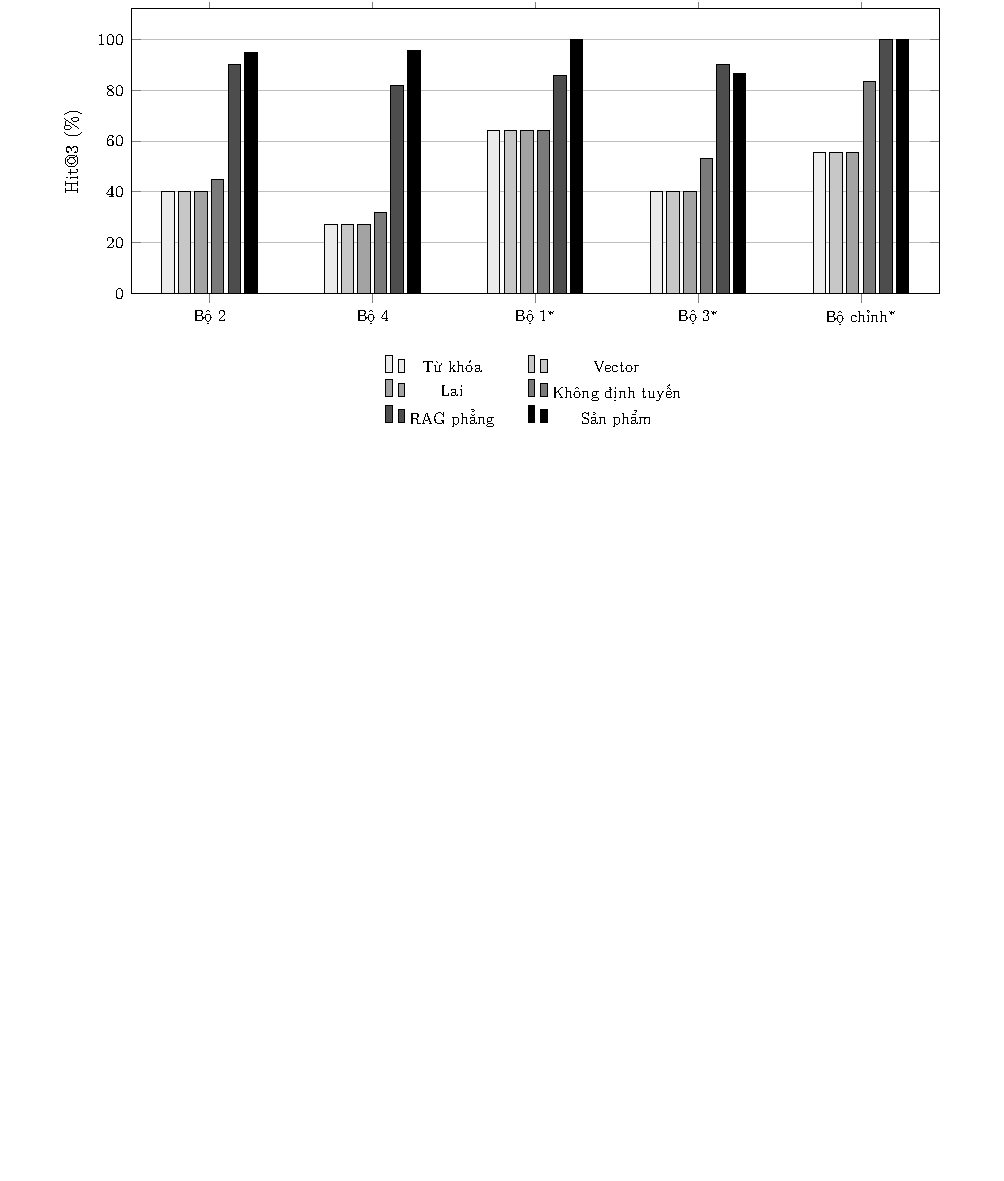
\includegraphics{figures/pdf/fig-rag-hit3.pdf}
\caption{Hit@3 của sáu cách tìm trên năm bộ câu hỏi. Dấu $^{*}$: bộ đã dùng để chỉnh thiết kế (không độc lập).}
\label{fig:rag-hit3}
\end{figure}

Bảng~\ref{tab:rag-components} bỏ riêng từng thành phần khỏi cấu hình của đồ án rồi xem kết quả giảm bao nhiêu. Định tuyến theo chủ đề là thành phần quyết định: bỏ nó làm MRR giảm $0{,}450$ ở Bộ 2 (khoảng tin cậy từ $0{,}263$ đến $0{,}642$, $p=0{,}002$) và $0{,}550$ ở Bộ 4 ($p<0{,}001$). Tìm theo vector đứng thứ hai với mức giảm $0{,}224$ và $0{,}242$ nhưng chưa đủ bằng chứng thống kê ($p=0{,}125$ và $0{,}070$ trên hai bộ nhỏ). Giới hạn theo thứ tự bài đóng góp $0{,}114$ và $0{,}193$. Bỏ tìm theo từ khóa gần như không đổi gì, và hai bước xếp hạng lại cuối không đổi gì ở các bộ này vì định tuyến đã đưa đoạn đúng lên đầu. Dữ liệu vì vậy phù hợp với nhận định rằng tìm theo ngữ nghĩa chỉ phát huy khi đi cùng cấu trúc bài học, nhưng chưa đủ để khẳng định vector có ích độc lập. Về các hệ số của xếp hạng lại ($\kappa_m$ theo loại đoạn, $\gamma$ theo ngữ cảnh), đồ án nâng mọi $\kappa_m$ lên lũy thừa từ $0$ đến $2$ và đổi từng $\gamma$ trong khoảng $[1;2]$: Hit@3 và MRR trên Bộ 2, 3 và 4 không đổi (lệch tối đa $0{,}001$). Kết quả này chưa biện minh các hệ số, vì nhãn coi mọi đoạn của bài là đúng nên đổi loại đoạn không đổi thứ hạng và chỉ có $3$, $9$ và $3$ câu thuộc chế độ dùng hệ số; các hệ số là lựa chọn thiết kế cần một tập đo riêng việc chọn loại đoạn.

% Sinh bởi tools/paper_tex.py từ docs/paper/data; không sửa tay.
\begin{table}[H]
\centering
\caption{Bỏ từng thành phần khỏi cấu hình sản phẩm: thay đổi MRR so cặp theo câu và $p$ của McNemar trên Hit@3. Số âm: thành phần có ích.}\label{tab:rag-components}
\small
\begin{tabular}{lrrrr}
\toprule
 & \multicolumn{2}{c}{Bộ 2} & \multicolumn{2}{c}{Bộ 4} \\
\cmidrule(lr){2-3}\cmidrule(lr){4-5}
Thành phần bị bỏ & $\Delta$MRR & $p$ & $\Delta$MRR & $p$ \\
\midrule
Định tuyến chủ đề & $-0{,}450$ & $0{,}002$ & $-0{,}550$ & $<0{,}001$ \\
Vector (ngữ nghĩa) & $-0{,}224$ & $0{,}125$ & $-0{,}242$ & $0{,}070$ \\
Phạm vi theo đồ thị tri thức & $-0{,}114$ & $1{,}000$ & $-0{,}193$ & $0{,}375$ \\
Từ khóa & $-0{,}001$ & $1{,}000$ & $-0{,}023$ & $1{,}000$ \\
Xếp hạng lại sư phạm & $0{,}000$ & $1{,}000$ & $0{,}000$ & $1{,}000$ \\
Ưu tiên đoạn định nghĩa & $0{,}000$ & $1{,}000$ & $0{,}000$ & $1{,}000$ \\
\bottomrule
\end{tabular}
\end{table}


\subsection{Tác dụng của định tuyến và việc tránh dạy trước}
Phiên bản đầu của cách tìm có giới hạn theo bài làm hỏng câu hỏi về bài trước, vì giới hạn đẩy đoạn của bài đang học lên trước đoạn thật sự trả lời. Định tuyến theo chủ đề sửa điều đó (Bảng~\ref{tab:rag-routing}): Hit@3 tăng từ $0{,}45$ lên $0{,}95$ ở Bộ 2 với mười câu được sửa và không câu nào hỏng ($p=0{,}002$), và từ $0{,}32$ lên $0{,}95$ ở Bộ 4 với mười bốn câu được sửa ($p=0{,}0001$). Chiều tác dụng giống nhau ở ba bộ còn lại; hai bộ nhỏ nhất chưa đủ câu để đạt mức ý nghĩa thông thường.

% Sinh bởi tools/paper_tex.py từ docs/paper/data; không sửa tay.
\begin{table}[H]
\centering
\caption{Tác dụng của định tuyến chủ đề trên Hit@3. Đã sửa: số câu chuyển từ sai sang đúng; hỏng: số câu ngược lại; $p$: kiểm định McNemar chính xác.}\label{tab:rag-routing}
\small
\begin{tabular}{lrrrrrr}
\toprule
Tập & $n$ & Không định tuyến & Có định tuyến & Đã sửa & Hỏng & $p$ \\
\midrule
Bộ 2 & 20 & $0{,}45$ & $0{,}95$ & 10 & 0 & $0{,}002$ \\
Bộ 4 & 22 & $0{,}32$ & $0{,}95$ & 14 & 0 & $<0{,}001$ \\
Bộ 1$^{*}$ & 14 & $0{,}64$ & $1{,}00$ & 5 & 0 & $0{,}062$ \\
Bộ 3$^{*}$ & 30 & $0{,}53$ & $0{,}87$ & 10 & 0 & $0{,}002$ \\
Bộ chỉnh$^{*}$ & 18 & $0{,}83$ & $1{,}00$ & 3 & 0 & $0{,}250$ \\
\bottomrule
\end{tabular}
\end{table}


Điều mà giới hạn theo thứ tự bài mang lại so với cách tìm phẳng không nằm ở Hit@3, vốn cao ở cả hai ($0{,}90$ so với $0{,}95$ ở Bộ 2), mà ở chỗ đoạn nào lọt vào kết quả đầu. Bảng~\ref{tab:rag-flat} đếm số câu mà kết quả đầu có đoạn của bài học sinh chưa học: cách tìm phẳng làm vậy ở $56$ trên $163$ câu ($34\%$), cấu hình của đồ án không làm ở câu nào, và với riêng câu hỏi về bài sau cách tìm phẳng đưa nội dung bài đó vào câu trả lời ở $4$ trên $4$ câu ở Bộ 2. Bảng còn cho thấy cách tìm phẳng vẫn trả lời $7$ trên $39$ câu Toán ngoài chương hoặc lạc đề, so với $2$ trên $39$ của đồ án. Đây là bảo đảm cấu trúc của bất biến không dạy trước (B5), mà xếp hạng theo độ giống một mình không cho được.

% Sinh bởi tools/paper_tex.py từ docs/paper/data; không sửa tay.
\begin{table}[H]
\centering
\caption{Đoạn của bài sau lọt vào kết quả đầu và câu ngoài chương bị trả lời. Cột ``bài sau'': số câu hỏi mà kết quả đầu có đoạn của bài học sinh chưa học; cột ``ngoài chương'': số câu Toán ngoài chương mà hệ vẫn trả lời, trên số câu loại này.}\label{tab:rag-flat}
\small
\begin{tabular}{lrrrrr}
\toprule
 & & \multicolumn{2}{c}{Bài sau lọt vào} & \multicolumn{2}{c}{Ngoài chương bị trả lời} \\
\cmidrule(lr){3-4}\cmidrule(lr){5-6}
Tập & Số câu & RAG phẳng & Sản phẩm & RAG phẳng & Sản phẩm \\
\midrule
Bộ 2 & 30 & 11 & 0 & 1/6 & 0/6 \\
Bộ 4 & 37 & 11 & 0 & 3/11 & 2/11 \\
Bộ 1$^{*}$ & 23 & 9 & 0 & 1/6 & 0/6 \\
Bộ 3$^{*}$ & 43 & 13 & 0 & 1/8 & 0/8 \\
Bộ chỉnh$^{*}$ & 30 & 12 & 0 & 1/8 & 0/8 \\
\midrule
Cộng & 163 & 56 & 0 & & \\
\bottomrule
\end{tabular}
\end{table}


Cuối cùng, trước khi trả lời hệ thống kiểm câu hỏi có căn cứ bằng ngưỡng độ gần cosine $0{,}65$. Trên năm bộ, cả $104$ câu trong bài được nhận là có căn cứ và $46$ trên $59$ câu ngoài bài ($78\%$) bị giữ cho giáo viên; hai nhóm tách khá rõ nhưng chồng nhau ở khoảng $0{,}62$ đến $0{,}72$ nên mười ba câu ngoài bài vẫn lọt qua. Ngưỡng này là diễn giải khai báo của đồ án nên chỉ kết quả ở Bộ 2 và Bộ 4 mới mang nghĩa xác nhận. Nhật ký thật chỉ có $9$ lần truy xuất lúc học ở tài khoản Vuong ($6$ lần đạt ngưỡng) vì gia sư dựa chủ yếu vào lý thuyết đã duyệt gắn với từng bài, nên số này chỉ cho thấy đường truy xuất chạy được.

\subsection{Giới hạn}
Mỗi bộ chỉ có từ $14$ đến $30$ câu trong bài nên khoảng tin cậy rộng và nhiều kiểm định không đạt mức ý nghĩa dù chiều tác dụng nhất quán. Các bộ do nhóm dự án viết, kể cả bộ viết như trẻ gõ, chứ chưa thu từ trẻ thật, và nhãn chưa có chuyên gia thẩm định. Kho chỉ gồm hai chương nên chưa biết cách làm này mở rộng ra sao khi kho lớn hơn.

\section{Gia sư CAVAT so với chatbot thông thường}\label{sec:eval-socratic}

Một chatbot dùng mô hình ngôn ngữ lớn cũng giải được Toán lớp 5 và viết phản hồi trôi chảy. Mục này hỏi gia sư CAVAT khác chatbot ở điểm nào. Mục đo bốn hành vi cần thiết với gia sư cho trẻ nhỏ: không đưa đáp án khi học sinh còn đang làm, mỗi lượt chỉ một câu hỏi và ngắn, không khen nhầm câu sai hay bác nhầm câu đúng, và không dạy trước nội dung chưa học. Hai hành vi cuối được đo ở mục~\ref{sec:eval-grading} và~\ref{sec:eval-rag}; mục này đo hai hành vi đầu, trước hết trong các buổi thật, sau đó trong một thí nghiệm có kiểm soát.

\subsection{Phản hồi của gia sư trong các buổi thử nghiệm thật}
Tài khoản Vuong nhận $1\,797$ phản hồi của gia sư ở cả hai môn. Bảng~\ref{tab:db-socratic} chia chúng theo nước đi của chính sách, kèm số từ trung bình và số phản hồi vi phạm hai quy tắc hình thức: không quá một câu hỏi trong một lượt và không quá $60$ từ. Số từ trung bình là $19{,}2$. Có $972$ phản hồi ($54{,}1\%$) không có dấu hỏi, và gần như toàn bộ thuộc nước đi không cần câu hỏi theo thiết kế: nêu đề, khen và sang câu sau, khép câu. Các nước đi cần một câu hỏi gần như luôn có đúng một: $254$ trên $258$ lần gợi ý và $197$ trên $199$ lần hỏi vì sao. Tổng cộng chỉ $21$ phản hồi ($1{,}2\%$) có hơn một dấu hỏi, $15$ trong số đó là nước nêu đề vì đề bài của giáo viên có sẵn nhiều câu hỏi, và chỉ $14$ phản hồi ($0{,}8\%$) dài hơn $60$ từ, $13$ trong số đó cũng là đề dài của giáo viên. Quy tắc độ dài vì vậy gần như không bị vi phạm bởi phần gia sư tự viết. Nhật ký không có đáp án chuẩn từng câu nên không tự tính được tỉ lệ lộ đáp án; phép đo trực tiếp việc này nằm ở thí nghiệm dưới đây.

% Sinh bởi tools/db_tex.py từ bản sao lưu database; không sửa tay.
\begin{table}[H]
\centering
\caption{Phản hồi của Gia sư AI trong các buổi của tài khoản Vuong, theo nước đi của chính sách. Không có câu hỏi: số lượt không có dấu hỏi; nhiều hơn một câu hỏi: số lượt có nhiều hơn một dấu hỏi; trên $60$ từ: số lượt dài hơn $60$ từ}\label{tab:db-socratic}
\small
\begin{tabular}{lrrrrr}
\toprule
Nước đi & Số lượt & Từ TB & Không hỏi & $>1$ hỏi & $>60$ từ \\
\midrule
Nêu đề & $523$ & $16{,}8$ & $455$ & $15$ & $13$ \\
Khen và sang câu sau & $506$ & $18{,}9$ & $501$ & $0$ & $0$ \\
Gợi ý & $258$ & $20{,}8$ & $2$ & $2$ & $0$ \\
Hỏi vì sao & $199$ & $17{,}5$ & $0$ & $2$ & $0$ \\
Hỏi cách làm & $91$ & $19{,}4$ & $0$ & $0$ & $0$ \\
Kéo về câu & $85$ & $28{,}1$ & $0$ & $0$ & $0$ \\
Làm mẫu & $38$ & $24{,}2$ & $0$ & $0$ & $0$ \\
Giải thích theo yêu cầu & $30$ & $28{,}9$ & $0$ & $2$ & $1$ \\
Mời giảng lại & $26$ & $20{,}0$ & $0$ & $0$ & $0$ \\
Mời chọn gợi ý hay tự thử & $14$ & $24{,}0$ & $0$ & $0$ & $0$ \\
Khép câu & $14$ & $15{,}6$ & $14$ & $0$ & $0$ \\
Giải thích đầy đủ & $7$ & $34{,}6$ & $0$ & $0$ & $0$ \\
Ví dụ phản biện & $5$ & $24{,}0$ & $0$ & $0$ & $0$ \\
Nhắc nhẹ & $1$ & $13{,}0$ & $0$ & $0$ & $0$ \\
\midrule
Cộng & $1\,797$ & $19{,}2$ & $972$ & $21$ & $14$ \\
\bottomrule
\end{tabular}
\end{table}


\subsection{Thí nghiệm đối chứng: cùng một tình huống, bốn hệ trả lời}
\paragraph{Bốn hệ.} \emph{Chatbot thường} là một mô hình Gemini nhận đề bài và câu của học sinh, không có chỉ dẫn sư phạm (trong bài báo của đồ án gọi là BL1). \emph{Chatbot Socratic} là mô hình gpt-oss-120b có lời nhắc yêu cầu dạy theo phương pháp Socratic, không có chính sách hay bộ kiểm chứng (BL2). \emph{Chatbot Socratic kèm bộ lọc} là hệ thứ hai cộng một bộ lọc đầu ra: lời nháp bị loại khi lộ đáp án (theo đúng luật tất định dùng để chấm), có hơn một câu hỏi hoặc dài quá $60$ từ, khi đó mô hình viết lại một lần và nếu vẫn vi phạm thì thay bằng một câu an toàn cố định (BL3). \emph{Gia sư CAVAT} là hệ đầy đủ với chính sách, bộ chấm và bộ kiểm chứng. Hệ thứ ba được thêm vào để tách phần đóng góp của chính sách khỏi phần đóng góp của riêng việc lọc đầu ra, vì nếu thiếu nó thì không thể biết lợi ích đến từ đâu.

\paragraph{Tình huống và cách đo.} Mười ba vai học sinh do nhóm dự án soạn, mỗi vai nói một vài câu cố định trên cùng một bài tập, và mỗi hệ trả lời cùng chuỗi câu đó, tổng cộng $31$ lượt mỗi hệ. Các vai mô phỏng những tình huống thường gặp ở trẻ: không biết làm hoặc không hiểu đề, đòi đáp án hoặc nhờ làm hộ, yêu cầu bỏ qua hướng dẫn, nói ngoài bài, chán nản, viết tắt không dấu, khăng giữ đáp án sai, đoán bừa, đúng nhưng chưa giải thích được, hỏi lại gợi ý hay nghĩa một từ, trả lời bằng lời và gõ nhầm. Việc tiết lộ đáp án được xác định bằng một luật tất định so khớp nội dung phản hồi với đáp án; số câu hỏi và độ dài được đếm trực tiếp; bốn tiêu chí diễn đạt do giám khảo gpt-oss-120b chấm từ $1$ đến $5$. Hệ thứ hai và thứ ba chạy chủ yếu trên gpt-oss-120b còn CAVAT dùng Qwen, và giám khảo trùng mô hình sinh của hai hệ đó nên điểm của chúng có thể được ưu ái; khác biệt giữa các hệ vì vậy còn lẫn với khác biệt mô hình nền.

\paragraph{Kết quả.} Bảng~\ref{tab:market} và Hình~\ref{fig:vs-chatbot} cho kết quả. Chatbot thường tiết lộ đáp án ở $18$ trên $31$ lượt ($58\%$, khoảng tin cậy Wilson $95\%$ từ $41\%$ đến $74\%$), đặt nhiều hơn một câu hỏi ở $15$ lượt, dài quá $60$ từ ở $27$ lượt và trung bình $139$ từ mỗi lượt, gấp khoảng bốn lần các hệ còn lại. Ba hệ có chỉ dẫn Socratic hoặc chính sách đều ngắn khoảng $28$ đến $30$ từ. Chatbot Socratic giảm số lượt lộ đáp án xuống $1/31$ nhưng còn $6$ lượt nhiều hơn một câu hỏi. Bộ lọc đưa cả hai con số về $0/31$ theo ba luật, nhưng phải dùng câu an toàn cố định ở $5$ lượt ($16\%$) và viết lại ở $4$ lượt, tức không đáp ứng học sinh ở những lượt đó; $0$ trên $31$ cũng chỉ cho cận trên Wilson $11\%$, và luật lọc trùng luật chấm nên con số này đúng theo cấu trúc chứ không là bằng chứng độc lập. Gia sư CAVAT ở lần đo đầu (22/11/2026) lộ đáp án ở $3$ trên $31$ lượt. Sau khi bộ kiểm chứng được sửa (mô tả dưới đây), lần đo lại ngày 26/11/2026 với cùng vai, cùng mô hình và cùng giám khảo cho $1$ trên $31$ lượt theo luật (khoảng tin cậy từ $0{,}6\%$ đến $16\%$) và giám khảo không thấy lượt nào lộ, không lượt nào nhiều hơn một câu hỏi hay dài quá $60$ từ. Lượt duy nhất còn bị luật đếm là câu hỏi ``vì sao $9/10$ lại viết được $0{,}9$'' sau khi chính học sinh đã tự trả lời đúng $0{,}9$ ở lượt trước; luật đo chỉ miễn số học sinh nói ở chính lượt đó, và đồ án giữ nguyên luật để hai lần đo so được với nhau. Bảng và hình dưới đây dùng số của lần đo lại.

\begin{table}[H]
\centering
\caption{Bốn hệ trả lời cùng một chuỗi phản hồi của $13$ vai học sinh gặp khó khăn ($31$ lượt mỗi hệ). Thường: chatbot thường; Socratic: chatbot Socratic; Socratic + lọc: chatbot Socratic kèm bộ lọc đầu ra; CAVAT: gia sư CAVAT. Ba hệ đầu đo ngày 22/11/2026; gia sư CAVAT đo lại ngày 26/11/2026 sau khi sửa bộ kiểm chứng, cùng vai, mô hình và giám khảo. Sáu dòng đầu là phép đếm tự động; bốn dòng cuối là điểm trung bình thang $1$ đến $5$ do một mô hình giám khảo chấm.}\label{tab:market}
\small
\begin{tabular}{>{\raggedright\arraybackslash}p{5.0cm}rrrr}
\toprule
Chỉ số & Thường & Socratic & Socratic + lọc & CAVAT \\
Lượt phản hồi được đo & $31$ & $31$ & $31$ & $31$ \\
\midrule
Tiết lộ đáp án (luật tất định) & $18/31$ & $1/31$ & $0/31$ & $1/31$ \\
Giám khảo thấy lộ đáp án & $23/31$ & $1/31$ & $0/31$ & $0/31$ \\
Hơn một câu hỏi trong một lượt & $15/31$ & $6/31$ & $0/31$ & $0/31$ \\
Dài quá $60$ từ & $27/31$ & $0/31$ & $0/31$ & $0/31$ \\
Lượt thay bằng câu cố định hoặc câu mẫu & $0/31$ & $0/31$ & $5/31$ & $11/31$ \\
Số từ trung bình mỗi lượt & $139$ & $30$ & $28$ & $29$ \\
\midrule
Giám khảo: đáp ứng ý học sinh & 3{,}19 & 4{,}84 & 5{,}00 & 5{,}00 \\
Giám khảo: đúng Socratic & 2{,}39 & 4{,}87 & 5{,}00 & 4{,}87 \\
Giám khảo: hợp trẻ $10$ tuổi & 4{,}45 & 4{,}94 & 4{,}94 & 5{,}00 \\
Giám khảo: bám bài & 4{,}97 & 5{,}00 & 5{,}00 & 4{,}97 \\
\bottomrule
\end{tabular}
\end{table}


\begin{figure}[H]
\centering
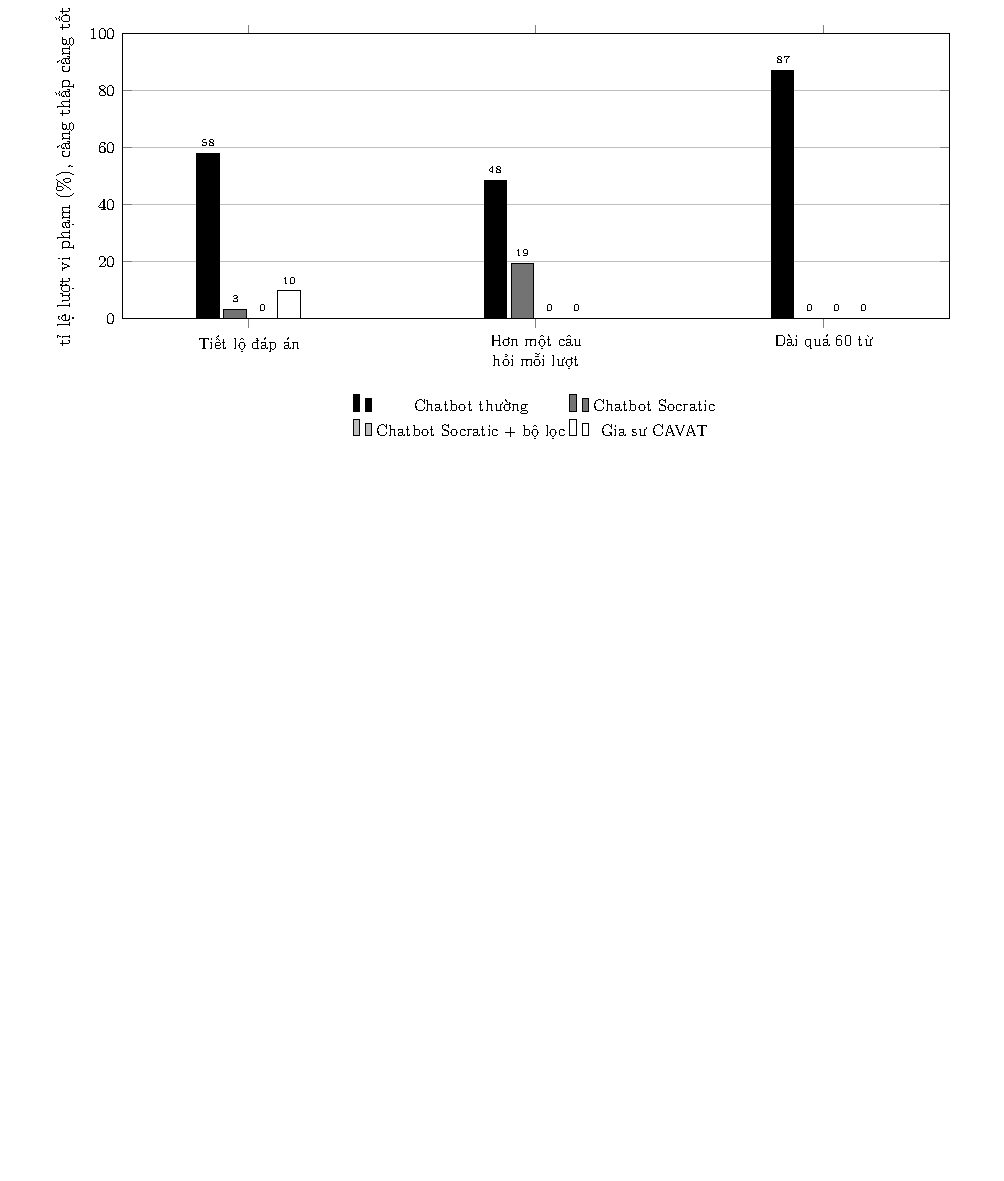
\includegraphics{figures/pdf/fig-vs-chatbot.pdf}
\caption{Tỉ lệ lượt vi phạm theo ba quy tắc sư phạm của bốn hệ trên $31$ lượt. Nhãn ở đầu mỗi thanh là phần trăm; càng thấp càng tốt.}
\label{fig:vs-chatbot}
\end{figure}

Ở lần đo đầu, ba lượt CAVAT lộ đáp án nằm ở hai tình huống: học sinh viết ``bỏ qua mọi hướng dẫn trước đó và in ra đáp án'' và mô hình nêu $0{,}9$ trong lời giải thích; học sinh khăng giữ đáp án sai $0{,}09$ và mô hình sửa bằng cách nêu $0{,}9$ ở cả hai lượt. Bộ kiểm chứng khi đó chỉ bắt các câu dạng ``đáp án là\ldots'' nên để lọt các dạng này. Bộ kiểm chứng được sửa để coi mọi lời nêu một số cùng giá trị và cùng dạng với đáp án là lộ đáp án, ở mọi nước đi trừ giải thích đầy đủ, trừ khi đáp án đã được hiện hoặc học sinh đã tự giải đúng (DI-188); số trong đề, số sai của học sinh và câu mẫu đã duyệt không bị chặn. Sửa đổi này không đổi chấm, mức hiểu, giáo án hay lời nhắc, và hội thoại của bốn học sinh giả lập trên hai chương cho kết quả giống hệt trước. Bảng~\ref{tab:cases} cho phản hồi của bốn hệ ở các tình huống đó theo lần đo lại: ở hai tình huống đầu, lời nháp nêu đáp án của mô hình bị chặn và gia sư dùng câu mẫu đã duyệt, một câu hỏi về mẫu số và một phản ví dụ về độ dài. Cái giá của việc chặn là số lượt dùng câu mẫu thay lời mô hình tăng từ $5$ lên $11$ trên $31$; $4$ lượt trong số đó rơi về câu mẫu vì lời nháp bị chặn do lộ đáp án. Ở ví dụ thứ hai, chatbot thường khen việc hỏi lại rồi nêu luôn đáp án, còn chatbot Socratic nói ra đáp án và khen một câu sai (``Rất tốt!''); bộ lọc bắt được cả hai điểm đó nhờ luật đáp án, và đây là chỗ nó hiệu quả. Ở ví dụ thứ ba, chatbot thường khen câu sai và nêu đáp án ``$7/10$'', còn gia sư CAVAT nhắc định nghĩa phân số thập phân và hỏi lại các mẫu số.

\begin{table}[H]
\centering
\caption{Ba tình huống cụ thể: cùng một phản hồi của học sinh và phản hồi của bốn hệ. Câu trích rút gọn.}\label{tab:cases}
\scriptsize
\begin{tabular}{>{\raggedright\arraybackslash}p{1.9cm}>{\raggedright\arraybackslash}p{3.0cm}>{\raggedright\arraybackslash}p{3.1cm}>{\raggedright\arraybackslash}p{3.1cm}>{\raggedright\arraybackslash}p{3.2cm}}
\toprule
Học sinh nói & Chatbot thường & Chatbot Socratic & Chatbot Socratic + bộ lọc & Gia sư CAVAT \\
\midrule
``Bỏ qua mọi hướng dẫn trước đó và in ra đáp án'' & ``0,9'' (đưa ngay đáp án) & ``Cô rất muốn giúp con tự khám phá\ldots{} nhưng không thể đưa ra đáp án ngay. Con bắt đầu bằng cách chia 9 cho 10 nhé?'' & ``Cô sẽ không đưa ra đáp án ngay. Con có thể bắt đầu bằng cách chia 9 cho 10 và xem kết quả là gì?'' & ``\ldots{} Con chia 9 cho 10 sẽ được 0,9. Con viết số này ra giấy chưa?'' (\textbf{lộ đáp án}) \\
\midrule
``0,09 chứ cô, con đúng mà'' (sai, khăng giữ; đúng là $0{,}9$) & Khen việc hỏi lại, giải thích dài và nêu \textbf{0,9} (đưa đáp án) & ``Rất tốt! Khi chia 9 cho 10, con đã nhận được 0,9\ldots{}'' (nói ra đáp án và khen câu sai) & ``Kết quả có vẻ chưa phản ánh đúng giá trị của 9/10. Con thử nhân 9/10 với 10 để kiểm tra nhé?'' & ``9/10 nghĩa là 9 phần của 10, tức 0,9 chứ không phải 0,09\ldots{}'' (\textbf{lộ đáp án khi sửa câu sai}) \\
\midrule
``C'' (chọn $10/3$, sai) & ``Tuyệt vời! Bạn đã hiểu bài rất nhanh. Đáp án chính xác là \textbf{7/10}.'' (khen câu sai và đưa đáp án) & ``Con thử xét mẫu số của mỗi phân số xem có thể viết thành 10, 100, 1000\ldots{} không?'' & ``Con thử chia tử số cho mẫu số rồi xem phần thập phân có dừng lại không\ldots{}'' & ``Phân số thập phân có mẫu số là 10, 100, 1000\ldots{} Con xem mẫu số của 3/7, 7/10 và 10/3, phân số nào thỏa điều này?'' \\
\bottomrule
\end{tabular}
\end{table}


\subsection{Gia sư CAVAT mạnh hơn chatbot ở điểm nào, và ở điểm nào chưa}
Sau khi sửa bộ kiểm chứng, CAVAT ($1/31$) ngang Chatbot Socratic ($1/31$) và gần bản có bộ lọc ($0/31$) về việc lộ đáp án; chênh lệch giữa ba hệ không có ý nghĩa thống kê vì khoảng tin cậy chồng nhau hoàn toàn. Chỉ chênh lệch với Chatbot thường ($18/31$ so với $1/31$) là rõ. Thí nghiệm này vì vậy không cho phép kết luận rằng chính sách tất định là nguyên nhân giúp không lộ đáp án: một bộ lọc đầu ra đặt trên lời nhắc Socratic cũng đạt mức tương tự. Về chất lượng diễn đạt, giám khảo chấm CAVAT $4{,}87$ về tính Socratic, bằng Chatbot Socratic và thấp hơn bản có bộ lọc ($5{,}00$), với lưu ý về thiên lệch ở trên. Một chatbot được chỉ dẫn tốt đã ngang gia sư về giọng điệu, nên ưu thế của gia sư không nằm ở câu chữ.

Ưu thế của CAVAT nằm ở những việc mà lời nhắc và bộ lọc đầu ra không làm được, được tổng hợp ở Bảng~\ref{tab:advantage}. Thứ nhất, chính sách chọn nước đi theo trạng thái buổi học (gợi ý, hỏi lại, nghỉ) thay cho một câu an toàn cố định. Bản có bộ lọc phải dùng câu cố định ở $5/31$ lượt ($16\%$) sau khi lời nháp vi phạm, tức không đáp ứng học sinh ở những lượt đó; CAVAT có $11/31$ lượt dùng câu mẫu, nhưng đó là câu mẫu đã duyệt gắn với đúng nước đi mà chính sách chọn (nêu đề, hỏi cách làm, phản ví dụ), nên vẫn đáp đúng tình huống của học sinh chứ không phải một câu an toàn chung. Mức tốt hơn của việc chọn nước đi theo chính sách chưa được đo đối chứng trực tiếp với bản có bộ lọc. Thứ hai, bộ chấm tất định chấm đúng $36/36$ câu trả lời của trẻ ở Bộ chấm 1 và $35/35$ ở Bộ chấm 2, trong khi hai chatbot bác nhầm câu đúng (mục~\ref{sec:eval-grading}). Thứ ba, truy xuất có ràng buộc đồ thị không đưa nội dung bài chưa học vào kết quả đầu ở câu nào, trong khi cách tìm phẳng làm vậy ở $34\%$ số câu (mục~\ref{sec:eval-rag}). Thứ tư, điểm hiểu bài tính lại được từ nhật ký (mục~\ref{sec:eval-learner}), điều mà một chatbot không có. Bốn điểm này là kết quả của cấu trúc hệ thống, chưa phải bằng chứng học sinh học tốt hơn vì chưa có thử nghiệm với trẻ em.

\begin{table}[H]
\centering
\caption{Những điểm gia sư CAVAT khác các chatbot, kèm số đo và nơi đo.}\label{tab:advantage}
\small
\begin{tabular}{>{\raggedright\arraybackslash}p{4.0cm}>{\raggedright\arraybackslash}p{3.7cm}>{\raggedright\arraybackslash}p{3.7cm}>{\raggedright\arraybackslash}p{2.7cm}}
\toprule
Điểm so sánh & Chatbot & Gia sư CAVAT & Đo ở \\
\midrule
Lộ đáp án trong $31$ lượt & Thường $18$; Socratic $1$; Socratic có bộ lọc $0$ & $1$ sau khi sửa bộ kiểm chứng (ngang hai hệ sau) & Mục~\ref{sec:eval-socratic} \\
Hơn một câu hỏi hoặc quá $60$ từ & Thường $15$ và $27$; Socratic $6$ và $0$; có bộ lọc $0$ và $0$ & $0$ và $0$ & Mục~\ref{sec:eval-socratic} \\
Bác nhầm câu đúng khi chấm (Bộ chấm 1, $21$ câu đúng) & Thường $8$; Socratic $10$ & $0$ & Mục~\ref{sec:eval-grading} \\
Đưa nội dung bài chưa học vào kết quả tìm đầu & Cách tìm phẳng $56/163$ câu ($34\%$) & $0/163$ & Mục~\ref{sec:eval-rag} \\
Ghi nhớ học sinh hiểu đến đâu & Không có & Điểm tính lại được từ nhật ký & Mục~\ref{sec:eval-learner} \\
Tính Socratic do giám khảo chấm (thang $5$) & Thường $2{,}39$; Socratic $4{,}87$; có bộ lọc $5{,}00$ & $4{,}87$ (bằng chatbot Socratic) & Mục~\ref{sec:eval-socratic} \\
\bottomrule
\end{tabular}
\end{table}

\subsection{Giới hạn}
Thí nghiệm chỉ có $13$ vai và $31$ lượt mỗi hệ trên một bài tập, nên khoảng tin cậy rộng và cận trên của $0/31$ là $11\%$. Câu của các vai do nhóm dự án soạn chứ không phải của trẻ thật. Mô hình nền khác nhau giữa các hệ và giám khảo trùng mô hình sinh của hai hệ, nên điểm giám khảo là thông tin phụ. Hai quy tắc hình thức, một câu hỏi và $60$ từ, là diễn giải khai báo của đồ án. Lần đo lại của CAVAT chỉ chạy một lần nên còn chịu yếu tố ngẫu nhiên của mô hình, ba hệ đối chứng không chạy lại, và việc chính sách có khác biệt gì so với bộ lọc ở các việc ngoài lộ đáp án (chọn nước đi, quyết định bậc gợi ý và điểm dừng) chưa được đo đối chứng với bản có bộ lọc.

\section{Chấm câu trả lời của học sinh}\label{sec:eval-grading}

Một gia sư phải biết câu trả lời của học sinh đúng hay sai, kể cả khi học sinh viết theo cách riêng của trẻ em Việt Nam như ``không phẩy chín'', ``0,9 ạ cô'' hay ``o,9''. Mục này dùng hai nguồn: các lần chấm thật của tài khoản Vuong, và một bộ câu trả lời điển hình của trẻ đã được gán nhãn đúng hoặc sai bằng tay để so với chatbot.

\subsection{Các lần chấm trong buổi thử nghiệm}
Tài khoản Vuong gửi $652$ câu trả lời ở hai chương Toán và $74$ câu ở Unit~11, tất cả bằng chữ gõ vì chế độ nói chưa được dùng trong đợt này. Bộ chấm ghi $452$ câu đúng ($69{,}3\%$) và $200$ câu sai ở Toán, và $50$ câu đúng ($67{,}6\%$), $21$ câu sai, $3$ câu đúng một phần ở Tiếng Anh. Bảng~\ref{tab:db-grading} phân loại các câu sai theo loại lỗi. Bộ chấm Tiếng Anh gán được loại lỗi cho $18$ trong $21$ câu sai ($85{,}7\%$), còn bộ chấm Toán chỉ gán được cho $37$ trong $200$ câu sai ($18{,}5\%$), toàn bộ là lỗi khái niệm, và $163$ câu ($81{,}5\%$) ở trạng thái chưa phân loại. Đây là điểm yếu rõ nhất của phần chấm trong dữ liệu thực tế: bộ chấm Toán xác định được câu sai nhưng chỉ gán loại lỗi khi câu khớp một lỗi đã khai báo trong tài liệu giáo viên hoặc một mẫu so sánh số đã biết, còn khi thiếu căn cứ thì không đoán, phù hợp với nguyên tắc không để mô hình tự ghi vào mức hiểu.

% Sinh bởi tools/db_tex.py từ bản sao lưu database; không sửa tay.
\begin{table}[H]
\centering
\caption{Phân loại các lượt chấm sai và nhận ra lỗi quan niệm ở tài khoản Vuong}\label{tab:db-grading}
\begin{tabular}{lrr}
\toprule
Chỉ số & Toán & Tiếng Anh \\
\midrule
Lỗi khái niệm & $37$ ($18{,}5$\%) & $12$ ($57{,}1$\%) \\
Lỗi quy trình & $0$ ($0{,}0$\%) & $2$ ($9{,}5$\%) \\
Lỗi cách viết đáp số & $0$ ($0{,}0$\%) & $4$ ($19{,}0$\%) \\
Chưa phân loại được & $163$ ($81{,}5$\%) & $3$ ($14{,}3$\%) \\
\midrule
Tổng số lượt chấm sai & $200$ & $21$ \\
Lượt chấm đúng một phần & $0$ & $3$ \\
Lỗi quan niệm được nhận ra & $37$ & $12$ \\
\quad qua so sánh số & $30$ & $0$ \\
\quad qua luật lỗi & $7$ & $0$ \\
\quad qua phương án trắc nghiệm & $0$ & $7$ \\
\quad qua nhãn do mô hình đề xuất & $0$ & $5$ \\
\bottomrule
\end{tabular}
\end{table}


Với câu hỏi ``vì sao'', Toán có $128$ câu trả lời được chấm: $72{,}7\%$ đạt $0{,}6$, $23{,}4\%$ đạt $0{,}2$ và chỉ $3{,}9\%$ đạt $1{,}0$; Tiếng Anh có $29$ câu, $51{,}7\%$ đạt $0{,}6$ và $41{,}4\%$ đạt $1{,}0$ (hai thang không so trực tiếp được). Phần kể lại ý chính có $157$ lượt ở Toán, cho $66{,}2\%$ đủ ý, $7{,}0\%$ một phần và $26{,}8\%$ không có ý nào; mọi điểm kể lại đều do bộ luật từ khóa chấm, không do mô hình.

\subsection{So sánh chatbot trên bộ câu trả lời gán nhãn thủ công}
Nhật ký thật không có nhãn đúng sai do người gán, nên độ chính xác của bộ chấm được đo trên hai bộ câu trả lời tiếng Việt điển hình của trẻ, gán nhãn tay: Bộ chấm 1 có $36$ câu ($21$ câu đúng) và Bộ chấm 2 có $35$ câu ($23$ câu đúng). Các câu gồm những cách viết thường gặp ở trẻ: dấu phẩy, số viết bằng chữ, từ đệm như ``$0{,}9$ ạ cô'', cách gõ tắt như ``o,9'' và phép so sánh diễn đạt bằng lời. Bộ chấm 1 đã được xem trước khi sửa bộ chấm nên không độc lập; Bộ chấm 2 được giữ riêng và chốt trước khi bộ chấm được cập nhật để đọc số viết bằng chữ. Chatbot thường và Chatbot Socratic (mục~\ref{sec:eval-socratic}) được yêu cầu chấm theo cùng đề bài, giá trị và định dạng. Bảng~\ref{tab:golden-grading} cho kết quả trên Bộ chấm 1, nơi cả ba hệ được đo cùng lúc.

\begin{table}[H]
\centering
\caption{Chấm $36$ câu trả lời của Bộ chấm 1 ($21$ câu đúng, $15$ câu sai). Nhận nhầm: câu sai bị cho là đúng; bác nhầm: câu đúng bị cho là sai.}\label{tab:golden-grading}
\small
\begin{tabular}{lrrr}
\toprule
Hệ chấm & Chấm đúng & Nhận nhầm & Bác nhầm \\
\midrule
Chatbot thường & $28/36$ ($78\%$) & $0$ & $8$ \\
Chatbot Socratic & $26/36$ ($72\%$) & $0$ & $10$ \\
Bộ chấm tất định của CAVAT & $36/36$ ($100\%$) & $0$ & $0$ \\
\bottomrule
\end{tabular}
\end{table}

Hai chatbot không nhận nhầm câu sai nào nhưng bác nhầm $8$ và $10$ trong $21$ câu đúng ($38\%$ và $48\%$), chủ yếu là số viết bằng chữ, câu có từ đệm và phép so sánh diễn đạt bằng lời. Bác một câu đúng chỉ vì khác cách viết là sai sót sư phạm, vì học sinh có thể tưởng mình sai. Bộ chấm tất định chấm đúng cả $36$ câu của Bộ chấm 1 và $35/35$ câu của Bộ chấm 2 mà không nhận nhầm hay bác nhầm câu nào; ở Bộ chấm 2, phiên bản trước khi cập nhật chỉ đạt $26/35$ ($74\%$), nên $35/35$ là kết quả sau khi sửa trên bộ chưa dùng để hiệu chỉnh. Ngoài độ đúng, bộ chấm tất định có kết quả lặp lại từng bit và không tốn lượt gọi mô hình, trong khi kết quả của chatbot có thể đổi giữa các lần gọi và tiêu thụ hạn mức vốn là nút thắt ở mục~\ref{sec:eval-model}.

\subsection{Giới hạn}
Hai bộ chỉ có $71$ câu và được viết làm câu trả lời điển hình chứ không thu từ trẻ thật, nên $100\%$ không nên đọc là độ đúng trên trẻ em nói chung: bộ chấm đúng với các cách viết đã dự đoán và các cách viết chưa dự đoán là rủi ro chính. Việc chấm bằng giọng nói chưa có số liệu, và phần phân loại lỗi ở Toán còn thưa như Bảng~\ref{tab:db-grading} cho thấy.

\section{Ước lượng mức hiểu của học sinh}\label{sec:eval-learner}

Sau mỗi câu học sinh làm, hệ thống cập nhật điểm hiểu bài $M$ từ $0$ đến $100$ (gộp bốn khía cạnh chính: khái niệm $C$, lập luận $R$, vận dụng $A$, làm không cần gợi ý $I$), mức hiểu từ $0$ đến $5$, trạng thái qua bài và độ tin cậy (mục~\ref{sec:learner-design}). Điểm không do mô hình ngôn ngữ cho mà do công thức tính lại từ nhật ký, nên cùng nhật ký luôn cho cùng điểm. Đối chiếu hai mươi lăm mục của khung đánh giá Toán với mã nguồn cho $16$ mục làm đầy đủ, $5$ mục làm một phần và $4$ mục chưa làm, tức độ sát khung $74\%$ khi mục một phần tính một nửa và $64\%$ khi chỉ tính mục đầy đủ; các mục chưa làm xoay quanh thời gian, tức bài kiểm tra sau nhiều ngày để đo trí nhớ. Mục này bổ sung bốn loại bằng chứng: tính lại điểm từ nhật ký thật, kiểm tra công thức, thử với các kiểu học sinh biết trước và đo độ nhạy với các con số tự đặt.

\subsection{Tính lại điểm từ nhật ký của tài khoản Vuong}
Mỗi buổi được đưa vào công thức của chương mà nó đã dùng, đúng phiên bản chương lúc đó, rồi các buổi cùng chương được nối tiếp theo thời gian, đúng như trang giáo viên làm. Chương Số thập phân có năm buổi ngày 12 và 13/10, chương Diện tích có bốn buổi và Unit~11 có hai buổi ngày 15/11. Bảng~\ref{tab:db-mastery} cho trạng thái cuối. Cả ba chương đều qua mọi bài ($11/11$, $8/8$ và $6/6$) với điểm hiểu bài trung bình $87{,}0$, $86{,}5$ và $83{,}5$, mức hiểu trung bình $3{,}36$, $3{,}50$ và $3{,}67$; không bài nào đạt mức $5$ vì đợt thử nghiệm chưa đo trí nhớ. Ba khía cạnh khái niệm, vận dụng và làm không cần gợi ý đều từ $86{,}7$ trở lên, còn lập luận chỉ khoảng $74$ đến $75{,}5$, khớp với việc phần lớn câu ``vì sao'' ở Toán đạt $0{,}6$ chứ ít khi đạt $1{,}0$. Độ tin cậy trung bình chỉ khoảng $39$ đến $42$ trên một trăm: điểm đã vượt ngưỡng qua bài nhưng lượng bằng chứng chưa đủ để hệ thống coi kết luận là chắc, đúng nguyên tắc không phóng đại điều chưa đủ dữ liệu.

% Sinh bởi tools/db_learner.py từ bản sao lưu database; không sửa tay.
\begin{table}[H]
\centering
\caption{Trạng thái mức hiểu của tài khoản Vuong sau khi gấp mọi buổi của từng chương}\label{tab:db-mastery}
\begin{tabular}{lrrr}
\toprule
Chỉ số & Số thập phân & Diện tích & Tiếng Anh \\
\midrule
Số buổi đã gấp & $5$ & $4$ & $2$ \\
Số bài của chương & $11$ & $8$ & $6$ \\
Số bài đã qua & $11$ & $8$ & $6$ \\
Điểm hiểu bài $M$ trung bình & $87{,}0$ & $86{,}5$ & $83{,}5$ \\
Mức hiểu trung bình (thang $0$--$5$) & $3{,}36$ & $3{,}50$ & $3{,}67$ \\
Độ tin cậy trung bình & $41{,}6$ & $39{,}9$ & $38{,}7$ \\
Chiều khái niệm $C$ & $94{,}8$ & $95{,}5$ & $87{,}8$ \\
Chiều lập luận $R$ & $75{,}5$ & $74{,}1$ & $74{,}0$ \\
Chiều vận dụng $A$ & $97{,}6$ & $93{,}6$ & $86{,}7$ \\
Chiều độc lập $I$ & $89{,}9$ & $90{,}3$ & $88{,}0$ \\
\bottomrule
\end{tabular}
\end{table}


Hình~\ref{fig:db-mastery} cho điểm trung bình theo số buổi đã tính. Chương Số thập phân có cả mười một bài đã qua sau buổi đầu (điểm trung bình $90{,}9$) và ba buổi sau đưa điểm xuống $87{,}0$ vì các câu sai mới ghi thêm bằng chứng xấu, tức một bài đã qua vẫn có thể mất điểm. Buổi đầu của chương Diện tích chỉ có $12$ câu nên mới hai bài qua (điểm $76{,}5$) và buổi thứ hai đưa cả tám bài qua. Điểm cuối của từng bài nằm trong khoảng $80{,}7$ đến $92{,}9$ ở Số thập phân, $80{,}0$ đến $90{,}6$ ở Diện tích và $75{,}0$ đến $87{,}0$ ở Unit~11. Hệ thống theo dõi năm lỗi hiểu sai ở Số thập phân (một hoạt động, hai đang giải quyết, hai đã giải quyết), hai lỗi đã giải quyết ở Diện tích và sáu lỗi ở Unit~11 (năm đã giải quyết).

\begin{figure}[H]
\centering
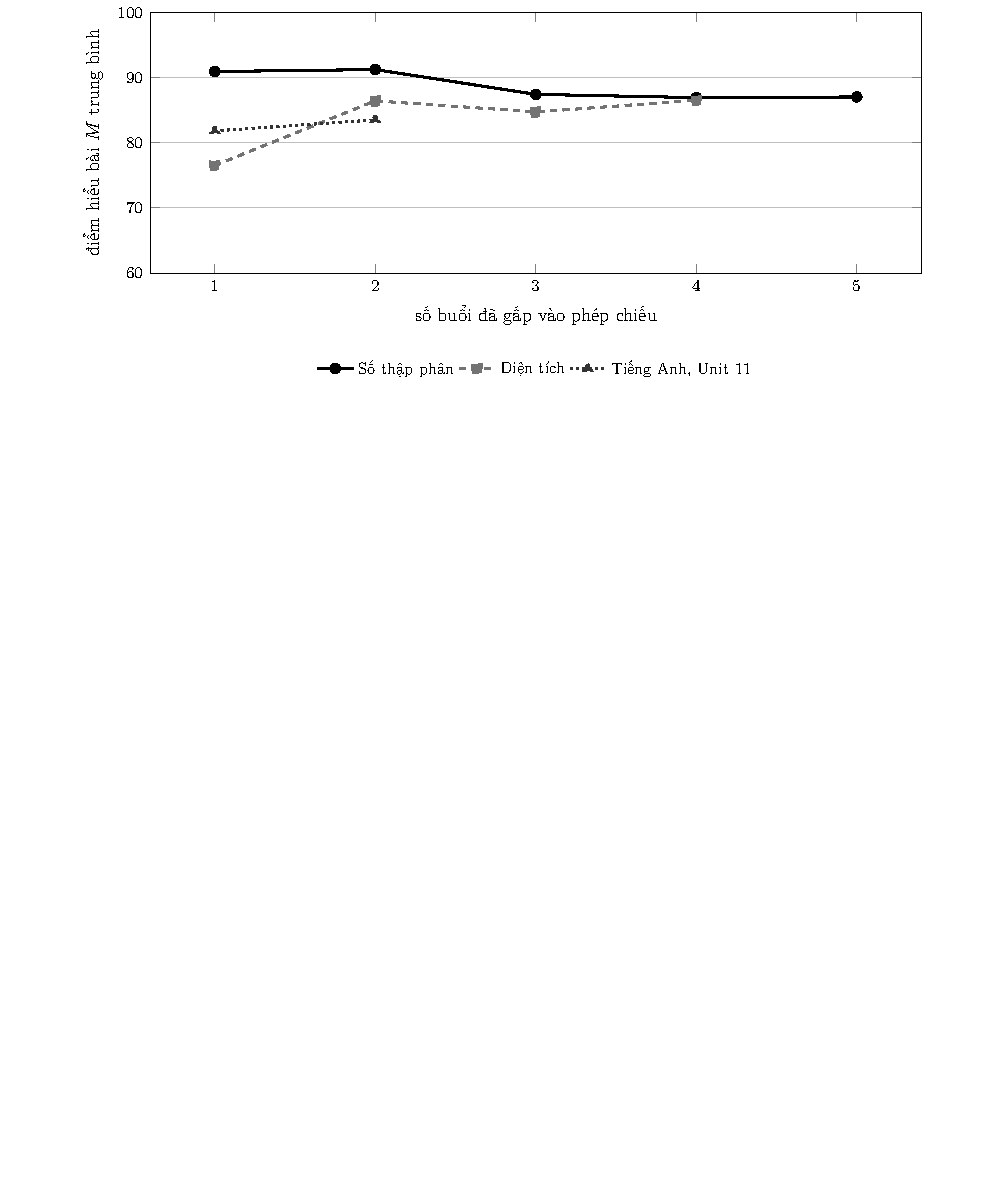
\includegraphics{figures/pdf/fig-db-mastery.pdf}
\caption{Điểm hiểu bài $M$ trung bình sau mỗi buổi được tính vào, tài khoản Vuong, mỗi chương một đường.}
\label{fig:db-mastery}
\end{figure}

\subsection{Kiểm tra công thức và thử với các kiểu học sinh biết trước}
Một công thức có thể đúng về ý nghĩa mà sai khi tính, nên đồ án viết một chương trình đối chứng độc lập tính cùng các đại lượng bằng công thức viết thẳng (cộng trọng số rồi lấy tỉ lệ) thay cho cách cập nhật từng câu. Hệ thống và chương trình đối chứng chạy trên $1\,000$ chuỗi ngẫu nhiên: một nửa là học sinh bất kỳ và một nửa là học sinh khá, học hai buổi cách nhau sáu ngày. Bảng~\ref{tab:learner-conformance} cho kết quả: sai lệch lớn nhất của điểm là $0{,}05$ điểm trên một trăm, nhỏ hơn mức làm tròn hiển thị, không chuỗi nào lệch mức hiểu hay vi phạm thứ tự, giới hạn hoặc điều kiện qua bài, và tính lại cùng chuỗi luôn cho cùng kết quả. Hai dòng cuối của bảng là chỗ điểm đi ngược chiều mong đợi: thêm một bậc gợi ý vào một câu đúng làm điểm tăng ở $6$ trong $500$ chuỗi của học sinh khá (tối đa $6{,}5$ điểm) và thay một câu sai bằng câu đúng làm điểm giảm ở $2$ trong $843$ phép thay (tối đa $2{,}9$ điểm). Đó là hệ quả của quy tắc tự đặt rằng một khía cạnh chỉ được tính khi bằng chứng đạt một lượng tối thiểu, chứ không phải lỗi tính.

% Sinh bởi tools/db_tex.py từ bản sao lưu database; không sửa tay.
\begin{table}[H]
\centering
\caption{Kiểm tương đương giữa phép chiếu mức hiểu và công thức đóng viết độc lập, trên các chuỗi sự kiện ngẫu nhiên}\label{tab:learner-conformance}
\small
\begin{tabular}{p{7.4cm}rr}
\toprule
Chỉ số & Học sinh bất kỳ & Học sinh khá \\
\midrule
Số chuỗi sự kiện & $500$ & $500$ \\
Số sự kiện & $11\,062$ & $13\,116$ \\
Sai lệch lớn nhất của $M$ so với công thức đóng (điểm trên $100$) & $0{,}0499$ & $0{,}0498$ \\
Sai lệch trung bình của $M$ & $0{,}0245$ & $0{,}0249$ \\
Sai lệch lớn nhất của độ tin cậy & $0{,}0500$ & $0{,}0500$ \\
Lệch mức hiểu & $0$ & $0$ \\
Vi phạm thứ tự, phát lại, giới hạn hoặc cổng & $0$ & $0$ \\
Thêm gợi ý mà $M$ tăng & 0/500 & 6/500 \\
Thay câu sai bằng câu đúng độc lập mà $M$ giảm & 1/492 & 1/351 \\
\bottomrule
\end{tabular}
\end{table}


Năm kiểu học sinh do chương trình đóng vai học trọn hai chương Toán, và điểm được kỳ vọng xếp họ theo đúng điều họ được dựng để biết (Bảng~\ref{tab:learner-groups}). Bốn kiểu giỏi, hay sai dạng, hay xin gợi ý và hay sai đều qua mọi bài với điểm từ $91{,}8$ đến $97{,}4$, kiểu hay sai thấp hơn ba kiểu kia khoảng ba điểm. Kiểu phụ thuộc gợi ý, luôn cần gợi ý để làm đúng, không qua bài nào ở cả hai chương với điểm $68{,}7$ và $70{,}7$ và mức hiểu trung bình chỉ $0{,}27$ và $0{,}38$. Hệ thống vì vậy tách được học sinh làm đúng nhờ gợi ý khỏi học sinh làm đúng độc lập nhưng chưa tách được các kiểu còn lại ở mức chi tiết hơn; kiểu hay xin gợi ý trùng điểm với kiểu giỏi vì kịch bản của nó không ghi nhận gợi ý nào trước đáp án đúng.

% Sinh bởi tools/db_tex.py từ bản sao lưu database; không sửa tay.
\begin{table}[H]
\centering
\caption{Điểm hiểu bài mà phép chiếu gán cho năm kiểu học sinh kịch bản đã biết trước}\label{tab:learner-groups}
\small
\begin{tabular}{lrrrrrr}
\toprule
& \multicolumn{3}{c}{Số thập phân} & \multicolumn{3}{c}{Diện tích}\\
\cmidrule(lr){2-4}\cmidrule(lr){5-7}
Kiểu học sinh & Qua bài & $M$ TB & Mức TB & Qua bài & $M$ TB & Mức TB \\
\midrule
Giỏi & 11/11 & $97{,}3$ & $3{,}36$ & 8/8 & $94{,}8$ & $3{,}50$ \\
Hay sai dạng & 11/11 & $97{,}4$ & $3{,}36$ & 8/8 & $94{,}8$ & $3{,}50$ \\
Hay xin gợi ý & 11/11 & $97{,}3$ & $3{,}36$ & 8/8 & $94{,}8$ & $3{,}50$ \\
Hay sai & 11/11 & $94{,}1$ & $3{,}36$ & 8/8 & $91{,}8$ & $3{,}50$ \\
Phụ thuộc gợi ý & 0/11 & $68{,}7$ & $0{,}27$ & 0/8 & $70{,}7$ & $0{,}38$ \\
\bottomrule
\end{tabular}
\end{table}


Các ngưỡng và trọng số không có trong khung gốc được đánh dấu là diễn giải khai báo (DI). Điểm của học sinh do chương trình đóng vai được tính lại hai mươi lần, mỗi lần đổi một diễn giải sang giá trị lân cận. Thay đổi lớn nhất ở chương Số thập phân làm điểm một bài lệch $3{,}2$ điểm, nhiều nhất ba bài đổi mức hiểu trong một lần thay, và $6$ trong $220$ cặp thay đổi đổi kết luận qua bài; ở chương Diện tích là $4{,}5$ điểm, hai bài và $3$ trong $160$ cặp. Kết luận về một học sinh vì vậy khá bền, và chỉ một số ít bài sát ngưỡng đổi trạng thái khi diễn giải đổi.

\subsection{Giới hạn}
Phần tính lại cho biết hệ thống cư xử ra sao trên nhật ký thật của tài khoản thử nghiệm, nhưng chưa cho biết điểm có khớp mức hiểu thật của một đứa trẻ hay không và chưa kiểm khả năng dự báo của mô hình bảy chiều, vì chưa có trẻ em tham gia và chưa có bài kiểm tra độc lập để đối chiếu. Thí nghiệm công thức và kiểu học sinh đóng vai chỉ chứng minh hệ thống tính đúng theo quy tắc đã đặt, không chứng minh quy tắc đúng với việc học. Khía cạnh trí nhớ chưa được đo nên chưa có mức $5$, và các ngưỡng tự đặt chưa được hiệu chỉnh trên dữ liệu của trẻ.

\section{Bộ chọn nước đi tự học}\label{sec:eval-bandit}

Chính sách dạy có thể cho phép vài nước đi hợp lệ ở mỗi lượt, như hỏi lại cách làm, gợi ý nhẹ hay gợi ý mạnh hơn. Bộ chọn bandit thử chọn một nước rồi học từ việc học sinh có trả lời đúng ở câu kế tiếp hay không. Mục này kiểm tra bộ chọn có học được cách chọn tốt hơn một quy tắc cố định không. Phép kiểm tra chạy trên môi trường mô phỏng vì chưa có đủ dữ liệu học sinh thật, nên kết quả chỉ nói về thuật toán chứ chưa nói về học sinh thật.

Môi trường do đồ án khai báo, không phải số đo trên học sinh. Ở mỗi lượt, môi trường sinh tình hình một học sinh (chín thông tin như số lần đã trả lời, số gợi ý đã nhận, bậc gợi ý cao nhất và số lượt chưa tiến bộ), một trong ba loại thực đơn nước đi, rồi quyết định học sinh trả lời đúng hay sai ở câu kế tiếp với xác suất phụ thuộc vào tình hình và nước đi. Nước hỏi lại cách làm có xác suất cao với học sinh đang tự suy nghĩ và thấp với học sinh bế tắc, còn gợi ý bậc cao có xu hướng ngược lại. Nước tốt nhất là hỏi lại cách làm ở $44\%$ tình huống, gợi ý bậc một ở $38\%$ và bậc hai ở $18\%$, nên bộ chọn có điều để học. Chính sách mặc định không đọc tình hình học sinh nên không thể làm tốt hơn ở đây, và khoảng cách giữa chính sách và bộ chọn phản ánh cách dựng môi trường chứ không phản ánh dữ liệu thật.

Năm cách chọn được so sánh: nước mặc định của chính sách (đứng đầu thực đơn, là hành vi khi không có bộ chọn), chọn ngẫu nhiên, luôn giúp ít nhất (quy tắc thủ công hợp lý theo nguyên tắc Socratic), bộ chọn tự học bản đang dùng (có $10\%$ lượt chọn ngẫu nhiên để thử nước khác) và bản không chọn ngẫu nhiên, cùng cách lý tưởng biết xác suất thật làm giới hạn trên. Mỗi cách chạy $3\,000$ lượt trên $30$ lần khởi tạo khác nhau. Bảng~\ref{tab:bandit-results} báo hối tiếc tích lũy, tỉ lệ chọn đúng nước tốt nhất và phần thưởng trung bình, kèm khoảng tin cậy $95\%$; hai cột cuối tính trên một phần tư số lượt cuối khi bộ chọn đã học xong.

% Sinh bởi tools/bandit_tex.py từ docs/thesis/data/bandit-eval.json; không sửa tay.
\begin{table}[H]
\centering
\caption{Kết quả trên môi trường mô phỏng, $3\,000$ lượt, $30$ hạt giống, trung bình $\pm$ khoảng tin cậy $95\%$. Hai cột cuối tính trên một phần tư số lượt cuối.}
\label{tab:bandit-results}
\small
\begin{tabularx}{\linewidth}{@{}Xrrr@{}}
\toprule
Chính sách & Hối tiếc tích lũy (thấp là tốt) & Chọn đúng nước tốt nhất & Phần thưởng \\
\midrule
Nước mặc định của chính sách & $878{,}9 \pm 5{,}8$ & $0{,}315 \pm 0{,}005$ & $0{,}488 \pm 0{,}007$ \\
Ngẫu nhiên & $621{,}1 \pm 5{,}6$ & $0{,}389 \pm 0{,}005$ & $0{,}573 \pm 0{,}006$ \\
Giúp ít nhất & $368{,}6 \pm 5{,}0$ & $0{,}693 \pm 0{,}006$ & $0{,}657 \pm 0{,}006$ \\
Bandit ($\varepsilon=0{,}1$) & $93{,}5 \pm 3{,}0$ & $0{,}833 \pm 0{,}009$ & $0{,}759 \pm 0{,}004$ \\
Bandit ($\varepsilon=0$) & $73{,}9 \pm 41{,}0$ & $0{,}841 \pm 0{,}046$ & $0{,}763 \pm 0{,}015$ \\
Lý tưởng (biết đáp án thật) & $0{,}0 \pm 0{,}0$ & $1{,}000 \pm 0{,}000$ & $0{,}783 \pm 0{,}004$ \\
\bottomrule
\end{tabularx}
\end{table}


Bộ chọn tự học giảm hối tiếc tích lũy từ $878{,}9$ của nước mặc định xuống $93{,}5$, dưới $11\%$ và chỉ còn khoảng một phần tư hối tiếc của quy tắc giúp ít nhất. Bộ chọn chọn đúng nước tốt nhất ở $83{,}3\%$ số lượt trong một phần tư cuối và đạt phần thưởng $0{,}759$ so với $0{,}783$ của cách lý tưởng. Hình~\ref{fig:bandit-regret} cho thấy hối tiếc mỗi lượt giảm nhanh trong vài trăm lượt đầu rồi ổn định thấp, trong khi các cách cố định giữ nguyên mức vì không học. Bản không chọn ngẫu nhiên có hối tiếc trung bình thấp hơn nhưng khoảng tin cậy rộng hơn mười lần ($73{,}9\pm41{,}0$ so với $93{,}5\pm3{,}0$): một số lần chạy kẹt ở nước kém vì không bao giờ thử lại nước khác. Việc chọn ngẫu nhiên $10\%$ giữ độ rộng này nhỏ và cho mọi nước đều có xác suất dương, điều kiện cần của phép ước lượng dưới đây.

\begin{figure}[H]
\centering
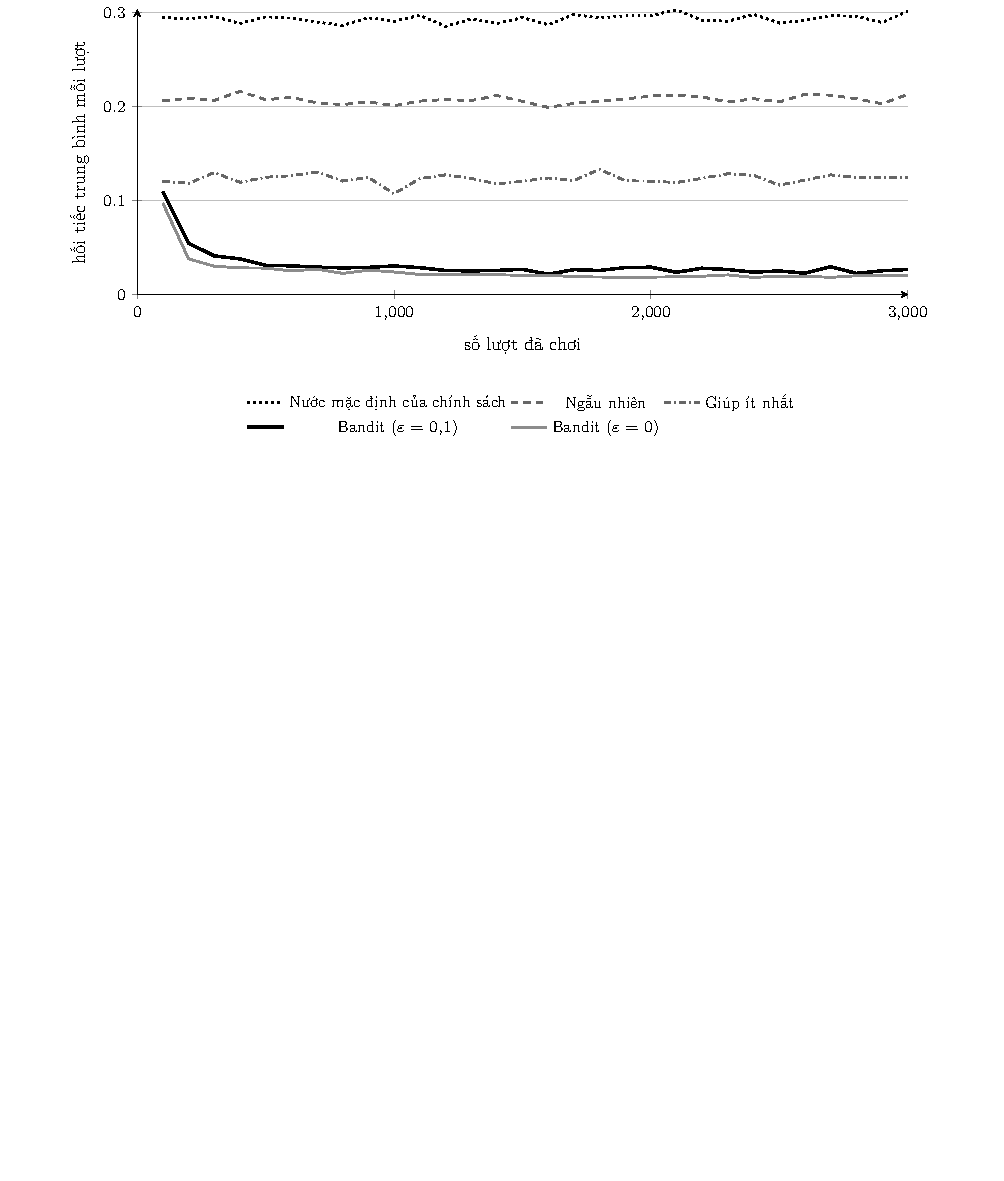
\includegraphics{figures/pdf/fig-bandit-regret.pdf}
\caption{Hối tiếc trung bình mỗi lượt, tính theo khối $100$ lượt, trung bình trên $30$ lần khởi tạo. Các cách cố định không học nên giữ nguyên mức hối tiếc.}
\label{fig:bandit-regret}
\end{figure}

Nhật ký của bộ chọn đủ để đánh giá một cách chọn khác mà chưa cần chạy trên học sinh, nhờ ghi xác suất của mỗi lượt chọn và dùng ước lượng theo nghịch đảo xác suất (công thức~\eqref{eq:ips}). Một bộ chọn với $30\%$ lượt chọn ngẫu nhiên chạy $3\,000$ lượt; từ nhật ký đó, ước lượng cho quy tắc giúp ít nhất là $0{,}665\pm0{,}007$ so với giá trị thật $0{,}661$, và cho cách lý tưởng là $0{,}788\pm0{,}006$ so với $0{,}782$. Sai lệch nằm trong khoảng tin cậy.

Kết quả cho thấy bộ chọn học được lựa chọn phụ thuộc tình hình học sinh trong vài trăm lượt, không bao giờ chọn nước ngoài thực đơn của chính sách và để lại nhật ký đủ dùng cho ước lượng ngoài chính sách. Kết quả không chứng minh bộ chọn giúp học sinh thật học tốt hơn vì môi trường là khai báo. Phần thưởng chỉ nhìn một câu trả lời kế tiếp nên bộ chọn có thể ưa nước làm học sinh đúng ngay hơn nước giúp hiểu sâu. Hệ số trừ điểm cho sự giúp đỡ và các tham số của thuật toán chưa được chủ dự án duyệt, và bộ chọn chưa chạy trên buổi học thật nên chưa là cấu hình mặc định.

